% LaTeX mintafájl szakdolgozat és diplomamunkáknak az
% SZTE Informatikai Tanszekcsoportja által megkövetelt
% formai követelményeinek megvalósításához
% Modositva: 2011.04.28 Nemeth L. Zoltan
% A fájl használatához szükséges a magyar.ldf 2005/05/12 v1.5-ös vagy késõbbi verziója
% ez letölthetõ a http://www.math.bme.hu/latex/ weblapról, a magyar nyelvû szedéshez
% Hasznos információk, linekek, LaTeX leirasok a www.latex.lap.hu weboldalon vannak.
%


\documentclass[12pt]{report}

%Magyar nyelvi támogatás (Babel 3.7 vagy késõbbi kell!)
\usepackage[utf8]{inputenc}
\usepackage{t1enc}
\usepackage[magyar]{babel}
% A formai kovetelmenyekben megkövetelt Times betûtípus hasznalata:
\usepackage{times}

%Az AMS csomagjai
\usepackage{amsmath}
\usepackage{amssymb}
\usepackage{amsthm}
\usepackage{mathtools}
\DeclarePairedDelimiter\floor{\lfloor}{\rfloor}

%A fejléc láblécek kialakításához:
\usepackage{fancyhdr}

%Természetesen további csomagok is használhatók,
%például ábrák beillesztéséhez a graphix és a psfrag,
%ha nincs rájuk szükség természetesen kihagyhatók.
\usepackage{graphicx}
\usepackage{psfrag}
\usepackage{algpseudocode}

%tetelszerû környezetek definiálhatók, ezek most fejezetenkent egyutt szamozodnak, pl.
\newtheorem{tet}{tetel}[chapter]
\newtheorem{defi}[tet]{Definíció}
\newtheorem{lemma}[tet]{Lemma}
\newtheorem{áll}[tet]{Állítás}
\newtheorem{köv}[tet]{Következmény}

%Ha a megjegyzések és a példak szövegét nem akarjuk dõlten szedni, akkor
%az alábbi parancs után kell õket definiální:
\theoremstyle{definition}
\newtheorem{megj}[tet]{Megjegyzés}
\newtheorem{pld}[tet]{Példa}

%Margók:
\hoffset -1in
\voffset -1in
\oddsidemargin 35mm
\textwidth 150mm
\topmargin 15mm
\headheight 10mm
\headsep 5mm
\textheight 237mm

%Egyéb, saját
\usepackage{hyperref}
\usepackage{listings,xcolor}
\usepackage{inconsolata}

\definecolor{mygreen}{HTML}{03AC13}
\definecolor{myblue}{HTML}{1338BE}
\definecolor{myyellow}{HTML}{FFD300}
\definecolor{myorange}{HTML}{FF8040}
\definecolor{myred}{HTML}{8D021F}
\definecolor{mypurple}{HTML}{9867C5}

\lstset{
  language        = php,
  basicstyle      = \small\ttfamily,
  keywordstyle    = \color{mypurple},
  stringstyle     = \color{myred},
  numbers         = left,
  numberstyle     = \color{myblue},
  identifierstyle = \color{mygreen},
  commentstyle    = \color{gray},
  emph            =[1]{php},
  emphstyle       =[1]\color{black},
  emph            =[2]{if,and,or,else},
  emphstyle       =[2]\color{myyellow},
  emph            =[3]{function},
  emphstyle       =[3]\color{myorange},
  emph            =[4]{require_once},
  emphstyle       =[4]\color{mypurple}
}



\graphicspath{ {./Fejezetek/Images/} }

\begin{document}
\newcommand*{\nfk}{\textbf{2NF}}%
\newcommand*{\nfh}{\textbf{3NF}}%
\newcommand*{\BCNF}{\textbf{BCNF}}%

%A FEJEZETEK KEZDÕOLDALAINAK FEJ ES LÁBLÉCE:
%a plain oldalstílust kell átdefiniálni, hogy ott ne legyen fejléc:
\fancypagestyle{plain}{%
%ez mindent töröl:
\fancyhf{}
% a láblécbe jobboldalra kerüljön az oldalszám:
\fancyfoot[R]{\thepage}
%elválasztó vonal sem kell:
\renewcommand{\headrulewidth}{0pt}
}

%A TÖBBI OLDAL FEJ ÉS LÁBLÉCE:
\pagestyle{fancy}
\fancyhf{}
\fancyhead[L]{Feladatgeneráló program készítése relációs adatmodell sémáinak normalizálásához}
\fancyfoot[R]{\thepage}


%A címoldalra se fej- se lábléc nem kell:
\thispagestyle{empty}

\begin{center}
\vspace*{1cm}
{\Large\bf Szegedi Tudományegyetem}

\vspace{0.5cm}

{\Large\bf Informatikai Intézet}

\vspace*{3.8cm}


{\LARGE\bf Feladatgeneráló program készítése relációs adatmodell sémáinak normalizálásához}


\vspace*{3.6cm}

%{\Large Diplomamunka}
{\Large Szakdolgozat}

\vspace*{4cm}

%Értelemszerûen megváltoztatandó:
{\large
\begin{tabular}{c@{\hspace{4cm}}c}
\emph{Készítette:}     &\emph{Témavezetõ:}\\
\bf{Félegyházi Dávid}  &\bf{Dr. Németh Gábor}\\
informatika szakos     &egyetemi adjunktus\\
hallgató&
\end{tabular}
}

\vspace*{2.3cm}

{\Large
Szeged
\\
\vspace{2mm}
2021
}
\end{center}


%A tartalomjegyzék:
\tableofcontents

%A \chapter* parancs nem ad a fejezetnek sorszámot
\chapter*{Feladatkiírás}
%A tartalomjegyzékben mégis szerepeltetni kell, mint szakasz(section) szerepeljen:
\addcontentsline{toc}{section}{Feladatkiírás}

Feladatgeneráló program készítése relációs adatmodell sémáinak normalizálásához

Az Adatbázisok kurzuson fontos hangsúlyt kap az relációs adatbázissémák normalizálása. A kurzus keretén belül, ebből a témakörből is zárthelyi dolgozatot írnak a hallgatók. Jelen szakdolgozati téma ezt hivatott segíteni.

A jelentkező feladata olyan Moodle plugin modul írása, amely az alábbi funkciókat látja el:
\begin{itemize}
    \item Feladatgenerálás különböző nehézségi szinten:
    \begin{itemize}
        \item relációs adatbázisséma és funkcionális függőséghalmaz generálása a feladatokhoz
    \end{itemize}
    \item A generált feladatok normalizálása 2. normálformába, 3. normálformába és Boyce-Codd normálformába.
    \item A feladatokat a Moodle felületén meg kell oldania a tanulónak, be kell tudni adni a megoldást, amelyet a rendszernek el kell tárolnia.
    \item A tanárnak látnia kell a beküldött feladatokat.
\end{itemize}
A hallgatói megoldások kiértékelését nem kell megvalósítani, azt egy másik program végzi.

\chapter*{Tartalmi összefoglaló}
\addcontentsline{toc}{section}{Tartalmi összefoglaló}

A tartalmi összefoglalónak tartalmaznia kell (rövid, legfeljebb egy oldalas, összefüggõ megfogalmazásban)
a következõket: a téma megnevezése, a megadott feladat megfogalmazása - a feladatkiíráshoz viszonyítva-,
a megoldási mód, az alkalmazott eszközök, módszerek, az elért eredmények, kulcsszavak (4-6 darab).

Az összefoglaló nyelvének meg kell egyeznie a dolgozat nyelvével. Ha a dolgozat idegen nyelven készül,
magyar nyelvû tartalmi összefoglaló készítése is kötelezõ (külön lapon), melynek terjedelmét a TVSZ szabályozza.

Relációsémák különböző nehézségek alapján generált feladatok és ezek megoldása egy általános megoldó algoritmussal, majd ezt egy local Moodle plug-inben történő implementálás. 
\chapter*{Bevezetés}
\addcontentsline{toc}{section}{Bevezetés}
A szakdolgozatom témája adatbázisok logikai relációs adatmodell szerinti példák generálása és megoldása, illetve egy gyakorló plugin elkészítése Moodle\footnote{Link:\href{https://moodle.org}{https://moodle.org}} rendszerben. Ezt PHP nyelven implementálom és építem be. A Moodle egy ingyenes és nyílt forráskódú oktatási tananyagkezelő rendszer, mely PHP-ben íródott és bárki számára használható és fejleszthető. Ebbe tudunk generálni saját oldalakat, készíthetünk saját adatbázist, tölthetünk fel fájlt, építhetünk bele saját weblapot vagy plugin-t, vagy akár más nyelvet is implementálhatunk bele, például JavaScript kódot. Emiatt elég elterjedt lett a különböző középiskolákban, illetve egyetemeken. Ráadásul, mivel egy webszerverről beszélünk, a cross-platform lehetősége is adott, sőt készítve lett egy Moodle applikáció Androidra és IOs-re is. Így összességében egy széles körben használható rendszer. \hfill \newline
A szakdolgozatban található adatbázissémákat 4 fajtára bontottam szét, amelyeket az alábbiak:\hfill \newline
\begin{itemize}
    \item Egyszerű: A relációs séma 7-9 attribútumot és 3 függést tartalmaz, melyek egyértelműen meghatározzák a séma \textbf{2NF}, \textbf{3NF} és \textbf{BCNF} alakját. Az első függés mindig egy részhalmaza a kulcsnak, amely egy nemkulcselemek egy részhalmazára mutat, a második az első függés jobboldali elemeinek egy részhalmazából egy még nem érintett nemkulcsbeli elemek egy részhalmazára mutat, illetve a harmadik függésben a teljes kulcs a maradék nemkulcsbeli elemekre mutat.
    \item Összetett: A relációs séma 7-8 attribútumot és 3 függést tartalmaz, viszont itt a függések baloldalai tartalmazhatnak nemkulcsbeli és kulcsbeli elemek párosításait is, illetve jobban oda kell figyelni a zártságra.
    \item Dupla: A relációs séma 9 attribútumot és 4 függést tartalmaz, melyekből 2 darab a \textbf{2NF}-et, 2 darab pedig a \textbf{3NF}-et sérti.
    \item Zártság: A relációs séma 7-8 attribútumot és 4 függést tartalmaz, viszont a séma \textbf{2NF} és \textbf{3NF} meghatározásához oda kell figyelni a sémát sértő függés bal oldalán lévő attribútumhalmaz zártságára, hogy ténylegesen megfeleljen.
\end{itemize}
Ezeket a példafeladatokat egy általános megoldó \textbf{2NF}, \textbf{3NF} és \textbf{BCNF} megoldóval értékelem ki és együttesen implementálom egy saját készítésű Moodle pluginben.\hfill \newline

Ezen algoritmusok elsajátítása fontos egy informatikus hallgató számára, mivel az adatok többszörös tárolását, redundancia elkerülését, ezáltal hatékonyabb adatbázis-struk-túra kialakítását lesznek képesek elsajátítani. Található az interneten több megoldó is, viszont ezek esetében nekünk kell megadni a feladatot, nincs benne generátor. Ezenkívül ilyen Moodle plugin jelenleg nem található a sablonok között, így ez jó lehet arra is, ha valaki ezt tovább akarja fejleszteni. Végezetül pedig készült egy másik, hasonló plugin is, amely egy normalizálási feladat diák által adott megoldását képes összehasonlítani a valódi megoldással és kiértékelni azt, így ezzel a pluginnel kombinálva egy tesztsegédprogram jöhet létre, melyet gyakorlásra és tesztírásra is lehet használni.

\chapter{Általános definíciók}
\section{Adatbázis, adatmodell}

\begin{defi}[Adat]
Az \textbf{adat} az elemi ismeret. Olyan számok, karakterek sorozata, melyhez nincs jelentés tulajdonítva. Onnantól, hogy tudjuk, mit jelent beszélhetünk \textbf{információ}ról. 
\end{defi}

Az adatokat szeretnénk értelmezni, könnyen kezelhető formába helyezni akár a programon kívül tároltatni. Erre szolgálnak az adatbázisok.

\begin{defi}[Adatbázis, sor, rekord]
Az \textbf{adatbázis} adott formátum és rendszer szerint tárolt adatok együttesét jelenti. Ennek alapvető adategységét \textbf{sor}nak vagy \textbf{rekord}nak hívjuk. Sor esetén egy teljes adatbázisbeli objektum értékét, míg rekord esetén egy objektum adott tulajdonságát értjük.
\end{defi}

\begin{defi}[Egyed,tulajdonság,kapcsolat]
\textbf{Egyednek} nevezzük azt az objektumot, amelyről szeretnénk adatokat tárolni. Ezeknek az egyedeknek egy-egy jellemzőjét \textbf{attribútum}nak hívjuk, illetve az egyedek között \textbf{kapcsolat}ok alakulhatnak ki, melyek meghatározhatják a különböző egyedek egyes tulajdonságait.
\end{defi}

Az adatokat szeretnénk rendszerezni is az adatbázisban, erre több módszer is szolgál, amelyek évek-évtizedek alatt alakultak ki. Ezen modellek a következők:
\begin{itemize}
    \item Hiearchikus modell
    \item Hálós modell
    \item Relációs modell
    \item Objektumorientált modell
    \item Objektum-relációs modell
\end{itemize}
A szakdolgozat a relációs modell-lel foglalkozik, amely a mai napig széles körben használt modell.

\begin{defi}[Relációs adatmodell]
A \textbf{relációs adatmodell}ben az adatokat és a köztük lévő kapcsolatokat kétdimenziós táblákban tárolja. A táblákban az azonos sorban álló egyedek alkotnak egy relációt. Az erre a modellre épülő adatbáziskezelő-rendszereket RDBMS-nek (Relational Database Management System) nevezzük.
\end{defi}

\begin{defi}[Relációs adatmodell attribútuma, attributumhalmaza, relációséma]
A relációs adatmodellben \textbf{attribútum}nak egy névvel és értéktartománnyal ellátott tulajdonságot nevezünk. A $Z$ attribútum értéktartományát $dom(Z)$-vel fogjuk jelölni, az angol "domain" szóból rövidítve. Egy relációs adatbázis attribútumainak összessége az \textbf{attribútumhalmaz}. Az attribútumhalmaz egy névvel ellátva pedig a \textbf{relációséma}. Legyen $A = \{A_1,\ldots,A_n\}$ egy attribútumhalmaz, és legyen a séma neve $R$, ekkor az a relációsséma jele $R(A_1,\ldots,A_n)$ rövidítve $R(A)$. Ha két séma, legyen $R$ és $S$ azonos attribútumokat is tartalmaz, akkor azt jelölhetjük $R.A_i$ és $S.A_i$-vel.
\end{defi}

\begin{defi}[$R(A)$ feletti $T$ reláció]
Az \textbf{$R(A)$ feletti $T$ reláció} alatt egy $T \subseteq dom(A_1) \times \ldots \times dom(A_n)$ halmazt értünk.  
\end{defi}

Viszont szeretnénk egy adattábla soraira egyértelműen tudjunk hivatkozni, ahhoz kell egy olyan attribútum, amely minden sorban különbözik. Erre fog szolgálni nekünk a kulcs.

\begin{defi}[Kulcs, szuperkulcs, egyszerű és összetett kulcs, elsődleges kulcs, külső kulcs]
A \textbf{szuperkulcs} az adattábla azon attribútumainak különleges tulajdonsága, mely egyértelműen meghatározza a tábla sorait. Formálisan  $R(A)$ sémában a $K \subseteq A$ halmaz szuperkulcs, ha bármely $R$ feletti $T$ tábla bármely két sora különbözik $K$-n. A szuperkulcs lehet a teljes sor is, de ebben az esetben minden egyes sorazonosítás esetén minden sort külön-külön meg kellene vizsgálni, amely nem praktikus. Emiatt célunk megkeresni azt a szuperkulcsot, mely a legkevesebb elemből áll. A \textbf{kulcs} az a szuperkulcs, melynek az elemszáma minimális, azaz egyetlen részhalmaza sem lesz szuperkulcs. Ha a kulcs egyelemű, akkor \textbf{egyszerű kulcs}ról, ha pedig többelemű, akkor \textbf{összetett kulcs}ról beszélünk. Az is megtörténhet, hogy egy adatbázisnak több kulcsa is van, ekkor érdemes kiválasztani egyet ezek közül és ez lesz az \textbf{elsődleges kulcs}. Ezenkívül pedig ha egy $R(A)$ egy $K\subseteq A$ részhalmaza egy másik relációs sémának az elsődleges kulcsaira mutat, akkor a $K$ \textbf{külső kulcs}.
\end{defi}

\begin{pld}
Vegyünk egy hétköznapi példát egy relációs adatbázis-modellre:
\begin{center}
    Könyv(\underline{ISBN}, \textit{kiadókód}, író, cím, megjelenés éve) \break
    Kiadó(\underline{kiadókód}, kiadó neve, város, cím)
\end{center}
Ebben a példában az ISBN egy attribútum, az $\{\text{ISBN, kiadókód, író, cím, megjelenés éve} \}$ egy attribútumhalmaz, Könyv a séma neve, $T = dom(\text{ISBN}) \times dom(\text{kiadókód})$ egy Könyv feletti $T$ reláció.
Szuperkulcs lehet például a $\{$ISBN, kiadókód, író, cím, megjelenés éve $\}$ vagy $\{$ISBN, kiadókód$\}$ vagy $\{$ ISBN $\}$. A kulcsa a Könyv relációsémának az ISBN (ezt mindig aláhúzással jelöljük), a Kiadónak pedig a kiadókód. Illetve a Könyv kiadókód attribútuma lesz egy külső kulcs.
\end{pld}

\section{Normálforma}

Ha minden adatot egy relációssémában tárolunk, az idő és tárigényes is lehet, mivel sokkal körülményesebb lehet a módosítás, törlés illetve a beszúrás. Emiatt egy nagyobb Relációsémát érdemesebb több, kisebb relációsémára bontani, amelyek kapcsolatban állnak egymással. Így időt és tárigényt csökkenthetünk, sőt az adattábláink is könnyebben átláthatóvá válnak. Erre szolgál a normalizálás. Viszont mielőtt ezt meg tudjuk tenni, elsőnek vezessünk be néhány alapdefiníciót.

\begin{defi} [Funkcionális függőség]
Legyen $R(A_1,\ldots,A_n)$ egy relációséma és $P,Q \subseteq \{A_1,\ldots,A_n\}$. Azt mondjuk, hogy $P$-től \textbf{funkcionálisan függ} $Q$ $(P \rightarrow Q)$, ha bármely $R$ feletti $T$ tábla esetén valahányszor két sor megegyezik $P$-n, mindannyiszor megegyezik $Q$-n is, azaz 
$\forall t_i, t_j \in T$ esetén $ t_i(P) = t_j(P) \Rightarrow t_i(Q) = t_j(Q)$. 
\end{defi}

\begin{defi}[Triviális/nemtriviális függés, teljesen nemtriviális függés]
Legyen $R(A_1,\ldots,A_n)$ egy relációséma és $P,Q \subseteq \{A_1,\ldots,A_n\}$. A $P \longrightarrow Q$ függést \textbf{triviális}nak nevezzük, ha $Q \subseteq P$, ellenkező esetben \textbf{nemtriviálisnak}. A $P \longrightarrow Q$ függést \textbf{teljesen nemtriviálisnak} nevezzük, ha $P \cap Q = \emptyset$.
\end{defi}

\begin{pld}
Vegyük az alábbi relációsémát:
\begin{center}
    Felhasználó(felhasználónév, e-mail, jelszó, születési év)
\end{center}
Ebben az alábbi függések a nemtriviálisak:
\begin{itemize}
    \item $\{\text{felhasználónév}\}\longrightarrow \{\text{e-mail}\}$
    \item $\{\text{felhasználónév}\}\longrightarrow \{\text{jelszó}\}$
    \item $\{\text{e-mail}\}\longrightarrow \{\text{felhasználónév}\}$
    \item $\{\text{e-mail}\}\longrightarrow \{\text{jelszó}\}$
    \item $\{\text{felhasználónév}\}\longrightarrow \{\text{e-mail,jelszó,születési év}\}$
\end{itemize}
Továbbá az alábbi függések teljesen nemtriviálisak:
\begin{itemize}
    \item $\{\text{felhasználónév,e-mail}\}\longrightarrow \{\text{jelszó}\}$
    \item $\{\text{felhasználónév, születési év}\}\longrightarrow \{\text{e-mail}\}$
    \item $\{\text{e-mail, jelszó}\}\longrightarrow \{\text{felhasználónév}\}$
\end{itemize}
\end{pld}

\begin{defi}[Attribútumhalmaz lezártja]
Egy $X$ \textbf{attribútumhalmaz lezártja} az $F$ függőségi halmaz szerint $X^+ = \{ A_i | X \longrightarrow A_i\}$ halmaz, tehát azon $A_i$ attribútumokból áll, melyekre az $X \longrightarrow A_i$ függőség $F$-ből levezethető.
\end{defi}

\begin{tet}[Attribútumhalmaz lezártjának kiszámítási módja] \label{closedAttribute}
Az alábbi algoritmus megadja egy $X$ attribútumhalmaz lezártját $F$ felett.
\begin{enumerate}
    \item Legyen $X^{(0)} = \{X\}$. Legyen $i = 0$.
    \item Keressünk egy $(P \longrightarrow Q) \in F$ függőséget úgy, hogy $P \subseteq X^{(i)}$ és $Q \not\subseteq X^{(i)}$. Ha nem találunk ilyet, akkor $X^+ = X^{(i)}$ és vége.
    \item Legyen $i = i + 1$ és $X_i = X_i \cup Q$, majd ugorjunk a $2.$ lépésre.
\end{enumerate}
\end{tet}

\begin{pld}
Vegyük az alábbi relációsémát a függőségeivel:
\begin{center}
    $R(a,b,c,d,e,f,g)$ \break
    $\{a\} \longrightarrow \{e,f\}$\break
    $\{f\} \longrightarrow \{g\}$\break
    $\{b\} \longrightarrow \{d\}$  
\end{center}
Ekkor $\{a,b\}$ lezártja:
\begin{itemize}
    \item $X^{(0)} = \{a,b\}.$
    \item $X^{(1)} = \{a,e,f\}$, mivel $\{a\} \longrightarrow \{e,f\}$ függőséggel tudjuk bővíteni.
    \item $X^{(2)} = \{a,e,f,g\}$, mivel $\{f\} \longrightarrow \{g\}$ függőséggel tudjuk bővíteni.
    \item $X^{(3)} = \{a,d,e,f,g\}$, mivel $\{b\} \longrightarrow \{d\}$ függőséggel tudjuk bővíteni.
    \item $X^{(4)} = \{a,d,e,f,g\} = X^{(3)}$ és az algoritmusnak vége.
\end{itemize}
\end{pld}

\begin{defi}[implied/nonimplied extraneous attribute]
Legyen $R(A)$ egy relációséma és $F$ függőségi halmaz, illetve $X,Y \subseteq A$ részhalmazok. Ekkor azt mondjuk, hogy egy $A_i$ \textbf{extraneous attribútum} egy $X \longrightarrow Y$ $F$ feletti függőségben, ha $A \in (A-A_i)^+$, Ha $A_i \in (A-A_i)^+$, akkor $A_i$ \textbf{implied extraneous attribútum}, viszont ha csak extraneous, de nem implied, akkor \textbf{nonimplied extraneous attribútum}.
\end{defi}

\begin{pld}
Vegyük $R(a,b,c)$ relációsémát és $\{a,b\} \longrightarrow \{c\}, \{a\} \longrightarrow \{c\}$ függőségeket. Ekkor $b$ nonimplied extraneous attribútum a $\{a,b\} \longrightarrow \{c\}$ függőségben. \hfill \break
Illetve vegyünk egy másik függőségi halmazt, melynek elemei $\{a,b\} \longrightarrow \{c\}, \{a\} \longrightarrow \{b\}$. Ekkor $b$ implied extraneous attribútum a $\{a,b\} \longrightarrow \{c\}$ függőségben.
\end{pld}

\begin{defi}[Fölösleges függőség]
Legyen $R(A)$ relációséma és $F$ függőségi halmaz, illetve $X,Y,Z \subseteq A$ részhalmazok. Ekkor azt mondjuk, hogy $X \longrightarrow Z$ \textbf{fölösleges függőség} $F$-ben, ha létezik egy olyan $Y \longrightarrow Z$, amely segítségével $X \longrightarrow Y \in F^+$.
\end{defi}

\begin{defi}[Teljes és részleges függőség]
Legyen $R(A)$ relációséma és $F$ függőségi halmaz, illetve $X,Y \subseteq A$ részhalmazok. Azt mondjuk, hogy $X \longrightarrow Y$ \textbf{teljes függőség}, ha bármely $A_i \in X$ elhagyása esetén az $X \longrightarrow Y$ már nem teljesülne. Ezenkívül $X \longrightarrow Y$ \textbf{részleges függőség}, ha $Y$ nem tartalmaz kulcs attribútumot és $B \in X$ elhagyása esetén a függés még mindig teljesül.
\end{defi}

\begin{defi}[Elsődleges és másodlagos attribútum]
Egy attribútumot \textbf{elsődleges attribútum}nak nevezünk, ha szerepel a relációséma valamely kulcsában, ellenkező esetben \textbf{másodlagos attribútum}nak hívjuk.
\end{defi}

\begin{defi}[Közvetlen és tranzitív függőség]
Legyen $X,Z \subseteq A$ úgy, hogy $X \rightarrow Z$. Azt mondjuk, hogy $X \longrightarrow Z$ \textbf{tranzitív függés}, ha létezik olyan $Y \subseteq A$, amelyre $X \longrightarrow Y$ és $Y \longrightarrow Z$ úgy, hogy az $Y \longrightarrow Z$ teljesen nemtriviális és $X$ nem függ $Y$-tól. Ellenkező esetben azt mondjuk, hogy $X \longrightarrow Z$ \textbf{közvetlen függés}.
\end{defi}

\begin{defi}[Normálformák]
Egy relációséma normálformái az alábbiak:
\begin{itemize}
    \item Egy relációséma \textbf{1NF}-ben van, ha az attribútumok értéktartománya csak egyszerű adatokból áll.
    \item Egy relációséma \nfk-ben van, ha minden másodlagos attribútum teljesen függ bármely kulcstól.
    \item Egy relációséma \nfh-ben van, ha minden másodlagos attribútum közvetlenül függ bármely kulcstól, azaz nincs kulcstól vett tranzitív függés.
    \item Egy relációséma \textbf{Boyce-Codd normálformá}-ban van (röviden \BCNF-ben), ha bármely nemtriviális $L \longrightarrow B$ függés esetén $L$ szuperkulcs.
\end{itemize}
\end{defi}

\begin{megj}
A szakdolgozat \nfk, \nfh és \BCNF normalizálással foglalkozik, de ezenkívül még létezik \textbf{4NF}, \textbf{ETNF}, \textbf{5NF}, \textbf{DKNF} és \textbf{6NF} normálformák is, viszont ezekre itt nem térek ki.
\end{megj}

\begin{tet}[A normálformák közti összefüggés]
Ha egy relációséma \BCNF-ben van, akkor \nfh-ben is, ha \nfh-ben van, akkor \nfk -ben is, illetve ha \nfk-ben van, akkor \textbf{1NF}-ben is. 
\end{tet}

\begin{pld}
Vegyük az alábbi relációsémát:
\begin{center}
    Reptér(\underline{név},\underline{város},ország, napi járatszám, főváros)
\end{center}
Illetve feleltessünk meg hozzá függőségeket is:
\begin{center}
    $\{\text{név,város}\} \longrightarrow \{\text{napi járatszám}\}$ \break
    $\{\text{város}\} \longrightarrow \{\text{ország, főváros}\}$ \break
    $\{\text{ország}\} \longrightarrow \{\text{főváros}\}$ 
\end{center}
Mivel minden attribútum elemi attribútumokból áll, ezért a relációs modell \textbf{1NF}-ben van. Viszont mivel egy város nevéből meg tudjuk hatázoni, hogy melyik országban van és mi a fővárosa, így nem minden másodlagos attribútum függ bármely kulcstól, tehát a $\{\text{város}\} \rightarrow \{\text{ország, főváros}\}$ függés sérti a \nfk-et. Emiatt ez a függőség alapján szét lehet bontani a relációs modellt az alábbira:
\begin{center}
    Reptér(\underline{név},\underline{város},napi járatszám) \break
    Helyezkedés(\textit{város}, ország, főváros)
\end{center}
Ha jobban megfigyeljük, látszik, hogy a városból adódik az ország és a főváros, de az országból meg tudjuk mondani annak fővárosát, így találhatunk ebben a modellben kulcstól vett tranzitív függést. Így a példánk tovább bontani a $\{\text{ország}\} \rightarrow \{\text{főváros}\}$ függés alapján, ami így néz ki:
\begin{center}
    Reptér(\underline{név},\underline{város},napi járatszám) \break
    Helyezkedés(\textit{város}, \textit{ország})\break
    Székhely(\underline{ország}, főváros)
\end{center}
és így teljesíti a \nfh-et is. Végezetül láthatjuk, hogy minden egyes másodlagos attribútum nemtriviális szuperkulcsbeli elemtől függ, emiatt a feladat már teljesíti a \BCNF-et.\hfill \break
Összegezve az példánk \BCNF alakja:
\begin{center}
    Reptér(\underline{név},\underline{város},napi járatszám) \break
    Helyezkedés(\textit{város}, \textit{ország})\break
    Székhely(\underline{ország}, főváros)
\end{center}
\end{pld}

\chapter{A feladatok generálása}

\section{Általános gondolat}
Mivel minden adatbázis más és más logika mentén épül fel, így az első dolog, amit meg kell valósítani, hogy a feladatok legyenek eltérőek. Ha véletlenszerű lenne a függéshalmaz generálása, abban az esetben létrejöhet könnyebben, szinte ránézésre megoldható és nehezebb, sokkal nagyobb rálátást igénylő feladat is. Emiatt érdemes sémákat készíteni, amelyeket felcímkézünk "könnyű", "közepes", illetve "nehéz" feladatokként, és ezek alapján készíteni a generátorokat. \par
A következő, amit érdemes figyelembe venni, hogy mennyi attribútumból és mennyi függőségből álljon egy relációs modell. Lehet olyan feladatokat is csinálni, ahol kevesebb függőség van, így olyan attribútumok is lesznek, amelyek egyik függésben sem szerepelnek, illetve lehet olyan is, ahol egy függőség könnyen levezethető egy másikból, vagy éppen csak nem fogjuk használni. Vegyük erre az alábbi példát: legyen $R(a,b,c)$ relációs séma, a függéshalmaz pedig a következő:
\begin{center}
    $\{a\} \longrightarrow \{c\}$, $\{b\} \longrightarrow \{c\}$, $\{a,b\} \longrightarrow \{c\}$
\end{center}
Ebben az esetben az $\{a,b\} \rightarrow \{c\}$ függés nem fog kelleni. Ez bonyolíthat egy feladatot, de nem fogja segíteni a normalizálás módszerét, így ezeket a típusú feladatokat nem fog generálni. \par
A következő 4 fajta feladattípus van megvalósítva:
\begin{itemize}
    \item Egyszerű, ahol a függésekből szinte azonnal látszik, hogy melyik fogja sérteni a \textbf{2NF} és \textbf{3NF} normálformát. Ezek a leggyakoribb példa- és tesztfeladatok így a diákok tudnak készülni ezen feladatok alapján.
    \item Dupla, ahol a függéseket 2 felé lehet venni és a két csoport egyértelműen mutatja a \nfk-et és \nfh-et sértő függéseket.
    \item Összetett, ahol több attribútum is szerepel a függések jobb-, illetve baloldalán. Ezek megoldása már igényel rutint és nem látszik egyértelműen, hogy hogyan kell felbontani az eredeti relációsémát.
    \item Zártság, ahol nem elég végignézni azt, hogy melyik függés sértheti a \nfk-et vagy a \nfh-et, hanem azt is meg kell vizsgálni, hogy ha azt a függés alapján szedjük szét, akkor tényleg a relációs modell teljesíti az adott normálformát.
\end{itemize}

Ezenkívül minden feladat esetén szabályokat vezetünk be, amely alapján történik a generálás. Ezek a szabályok:
\begin{itemize}
    \item Mennyi attribútumból álljon feladat,
    \item Mennyi kulcsa legyen a relációsémának,
    \item Legyen-e több elsődleges elem, mint amennyi kulcselem van,
    \item Mennyi függésből álljon, azok teljes vagy részleges függések legyenek-e,
    \item Az egyes függések milyen logika mentén legyenek felépítve, illetve mennyi elem legyen a bal- és jobboldalakon. 
\end{itemize}
Végezetül pedig vezessünk be pár jelölést:
\begin{itemize}
    \item $Fg\rightarrow Bo, Fg \rightarrow Jo$ egy függés bal-, és jobboldala.
    \item $K$ a kulcsok halmaza
\end{itemize}

\section{Egyszerű feladat bemutatása}

\subsection{Általános szemlélet}
Egyszerűbb feladat esetén a függések vizsgálatánál is egyértelműen fog látszani, hogy melyek lehetnek sértőek a \nfk-re, \nfh-re és a \BCNF-re.
\begin{pld}
    Legyen $R(\underline{a},b,c,d,e,f,\underline{g})$ és legyen $F$:
    $$
    \begin{matrix}
    \{a\} & \longrightarrow & \{b,d,e\}\\
    \{a,g\} & \longrightarrow &  \{f\} \\
    \{d,e\}  & \longrightarrow & \{b,c\}
    \end{matrix}
    $$
    
    és tegyük fel, hogy teljesül az \textbf{1NF}. Ekkor látszik, hogy az $\{a\} \rightarrow \{b,d,e\}$ függés sérti a \nfk-t, mivel nem minden másodlagos attribútum függ teljesen bármely kulcstól. Emiatt ezen függés felbontása esetén kapjuk az alábbi felbontást:
    \begin{center}
        $R_1(\underline{a},f,\underline{g})$ \break
        $R_2(\underline{a},b,c,d,e)$
    \end{center}
    A \textbf{3NF} esetén látni lehet, hogy $\{a\} \rightarrow \{b,d,e\}$ és $\{d,e\} \rightarrow \{b,c\}$ fogja sérteni, mivel található tranzitív függés az attribútumok közt. Emiatt a \nfh-nek megfelelő relációs modell
    \begin{center}
        $R_1(\underline{a},f,\underline{g})$ \break
        $R_2(\underline{a},\underline{d},\underline{e})$ \break
        $R_3(b,c,\underline{d},\underline{e})$
    \end{center}
    alakú. \par
    A \textbf{BCNF} alakra hozáshoz pedig a relációs modellt nem kell változtatni, mivel $R1$ az $\{a,g\} \rightarrow \{f\}$ függésből, $R2$ az $\{a\} \rightarrow \{d,e\}$ függésből, illetve $R3$ a $\{d,e\} \rightarrow \{b,c\}$ függésből adódik.
\end{pld}
A példán keresztül látható, hogy minden függést felhasználunk, illetve minden függés egyértelműen meghatározza, hogy melyik normálformát sérti. Emiatt ez a feladat jó gyakorló feladat lehet.

\subsection{Generáló algoritmus}

Az egyszerű feladat esetén a szabályok meghatározása a következő:
\begin{itemize}
    \item $7-9$ attribútuma legyen a relációnak,
    \item $\floor*{\frac{n}{3}}$ darab kulcs legyen, ahol $n$ attribútumok száma,
    \item kulcsok halmaza egyezzen meg az elsődleges attribútumok halmazával,
    \item $3$ függésből álljon: kettő részleges, egy teljes függésből,
    \item $1.$ függés: $\big\{ a_i \in A \big| a_i \text{ kulcselem}  \big\} \longrightarrow \big\{  a_i \in A \big| a_i \text{ nem kulcselem}  \big\}$ 
    \item $1. $ függés: $\big \{ 1 \text{ és } (|K|-1) \text{ közötti elem} \big\} \longrightarrow \big\{ n-5 \text{ db elem} \big \}$
    \item $2.$ függés: $\big\{ a_i \in A \big| a_i \in 1.Fg \rightarrow Jo  \big\} \longrightarrow \big\{  a_i \in A \big| a_i \in A \backslash (K \cup 1.Fg \rightarrow Jo)  \big\}$ 
    \item $2. $ függés: $\big \{ 1 \text{ és } (1.Fg\rightarrow Jo - 1) \text{ közötti elem} \big\} \longrightarrow \big\{ 1 \text { és } ( (|A \backslash (K \cup 1.Fg \rightarrow Jo)| - 1)  \text{ közötti elem} \big \}$
    \item $3.$ függés: $\big\{ K \big\} \longrightarrow \big\{  a_i \in A \big| a_i \not\in (1.Fg \cup 2.Fg)  \big\}$ 
    \item $3. $ függés: $\big \{ |K| \text{ db elem} \big\} \longrightarrow \big\{|A \backslash (1.Fg \cup 2.Fg)| \text{ db elem} \big \}$
\end{itemize}

Azáltal, hogy az attribútumszám és a függéseken belüli elemszámok nem állandóak, a gondolatmenet kevésbé kiismerhető, csak kellő idővel, de addigra már a tanuló meg is tanulta a tananyagot. 

\section{Dupla feladat bemutatása}

\subsection{Általános szemlélet}
Dupla feladat esetén a megoldáshoz nem csak egy függés van, amely sérti a \nfk-et és a \nfh-et. Így elsődleges feladata ennek a típusnak, hogy a diák ne csak keressen egy függést, amely sérti a normálformákat, hanem ellenőrizze, hogy az adott relációs modell már teljesíti-e, vagy még mindig van-e benne sértő függés.
\begin{pld}
    Legyen $R(a,\underline{b},c,\underline{d},e,f,g,h,\underline{i})$ és legyen $F$:

    $$
    \begin{matrix}
    \{b,i\} & \longrightarrow & \{a,e,h\}\\
    \{d\} & \longrightarrow &  \{c,e,g,f\} \\
    \{c,f\}  & \longrightarrow & \{e,g\} \\
    \{h\}  & \longrightarrow &\{a\} 
    \end{matrix}
    $$
    és tegyük fel, hogy teljesül az \textbf{1NF}. Ekkor láthatjuk, hogy a  $\{b,i\} \longrightarrow \{a,e,h\}$ sérti a \nfk-t, így e mentén bontva a relációs modellt a következő jön létre:
    \begin{center}
        $R_1(a,\underline{b},e,h,\underline{i})$ \break
        $R_2(\underline{b},c,\underline{d},f,g,\underline{i})$
    \end{center}
    Viszont látható, hogy $R_2$ még mindig nincs \nfk-ben, mert sérti $\{d\} \longrightarrow \{c,g,f\}$. Így e mentén felbontjuk $R_2$-t:
    \begin{center}
        $R_1(\underline{b},\underline{d},\underline{i})$\break
        $R_2(a,\underline{b},e,h,\underline{i})$ \break
        $R_3(c,\underline{d},f,g)$\break
    \end{center}
    és így minden séma \nfk-ben van.\par
    \textbf{3NF} esetén a $\{c,f\} \longrightarrow \{g\}$ és a $\{h\} \longrightarrow \{a\}$ függések is sértik. Így ezek alapján a felbontás:
    \begin{center}
        $R_1(\underline{b},\underline{d},\underline{i})$\break
        $R_2(\underline{b},e,\underline{h},\underline{i})$ \break
        $R_3(\underline{c},\underline{d},\underline{f})$\break
        $R_4(\underline{c},\underline{f},g)$\break
        $R_5(a,\underline{h})$\break
    \end{center}
    és így minden séma \nfh-ban van.\par
    Illetve észrevehető, hogy a minden relációséma egy függésből ered, amelynek a szuperkulcsai a függések baloldalai, így minden séma \BCNF-ben van.
\end{pld}

\subsection{Generáló algoritmus}

A dupla feladat esetén a következő szabályokat tartjuk be:
\begin{itemize}
    \item $9$ attribútuma legyen a relációnak,
    \item $3$ darab kulcs legyen,
    \item kulcsok halmaza egyezzen meg az elsődleges attribútumok halmazával,
    \item $4$ függésből álljon: négy részleges függésből,
    \item $1.$ függés: $\big\{ a_i \in A \big| a_i \text{ kulcselem}  \big\} \longrightarrow \big\{  a_i \in A \big| a_i \text{ nem kulcselem}  \big\}$ 
    \item $1.$ függés: $\big \{ (|K|-1) \text{ db elem} \big\} \longrightarrow \big\{ 3 \text{ és } 4 \text{ közötti elem} \big \}$
    \item $2.$ függés: $\big\{ a_i \in A \big| a_i \in 1.Fg \rightarrow Jo  \big\} \longrightarrow \big\{  a_i \in A \big| a_i \in (1.Fg \rightarrow Jo \backslash 2.Fg \rightarrow Bo)  \big\}$ 
    \item $2.$ függés: $\big \{ 1 \text{ és } (1.Fg\rightarrow Jo - 1) \text{ közötti elem} \big\} \longrightarrow \big\{ 1 \text { és } |(1.Fg \rightarrow Jo \backslash 2.Fg \rightarrow Bo)|  \text{ közötti elem} \big \}$
    \item $3.$ függés: $\big\{ K \backslash 1.Fg\rightarrow Bo \big\} \longrightarrow \big\{  a_i \in A \big| a_i \in (R \backslash 1.Fg)  \big\}$
    \item $3.$ függés: $\big \{ 1 \text{ db elem} \big\} \longrightarrow \big\{|A \backslash (K \cup 1.Fg \rightarrow Jo) \text{ db elem} \big \}$
    \item $4.$ függés: $\big\{ a_i \in A \big| a_i \in 3.Fg\rightarrow Jo \big\} \longrightarrow \big\{ 3.Fg\rightarrow Jo \backslash 4.Fg\rightarrow Bo\big\}$
    \item $4.$ függés: $\big \{ 1 \text{ és } (3.Fg\rightarrow Jo - 1) \text{ közötti elem} \big\} \longrightarrow \big\{ 1 \text { és } |(A \ (K \cup 1.Fg \rightarrow Jo \cup 4.Fg \rightarrow Bo)|  \text{ közötti elem} \big \}$
\end{itemize}

Azáltal, hogy a függéseken belüli elemszámok nem állandóak, a gondolatmenet kevésbé kiismerhető. Ennél a generátornál a sémára könnyebben rá lehet ismerni, ha valaki ismeri az egyszerű feladatok gondolatmeneteit, viszont ennek ellenére is ad újat a tanulóknak.

\section{Összetett feladat bemutatása}

\subsection{Általános szemlélet}

Ennél a feladattípus csak azoknak ajánlatos, akik a másik két feladatot meg tudták csinálni. Ami miatt ez a feladattípus nehezebb, mint az előzőek, érdemes megvizsgálni az attribútumok elhelyezkedését. Legyen $ls$ azon attribútumok halmaza, amelyek csak a függőségek bal oldalán található, $rs$ amelyek csak a jobb oldalon és $lr$ pedig amelyek mindkét helyen.
Egyszerű feladat esetén:
\begin{center}
    $ls = \{$a,g$\}$ \break
    $rs = \{$b,c,f$\}$ \break
    $lr = \{$d,e$\}$
\end{center}
Dupla feladat esetén: 
\begin{center}
    $ls = \{$b,d,i$\}$ \break
    $rs = \{$a,e,g$\}$ \break
    $lr = \{$c,f,h$\}$
\end{center}

Mindkét esetben látszik, hogy $ls$ a kulcsok halmaza lesz, $lr$ pedig azok az elemeket tartalmazza, melyek azon függőségek bal oldalán található, amely sérti a \nfh-et. Ha ezt a gondolatot ismerjük, akkor elég gyorsan meg tudjuk csinálni ezeket a feladattípusokat.
Viszont az Összetett feladat esetén más lesz a helyzet:

\begin{pld}
Legyen $R(\underline{a},b,\underline{c},d,e,f,g)$ és legyen $F$:
\begin{center}
    $\{a\} \longrightarrow \{d,e\}$ \break
    $\{c,e\} \longrightarrow \{b,f\}$ \break
    $\{d,f\} \longrightarrow \{g\}$ \break
\end{center}
A \nfk-re hozáshoz elsőnek a $\{a\} \longrightarrow \{d,e\}$ függés alapján kell egy darabolást csinálni a relációos modellen, így pedig
\begin{center}
    $R_1(\underline{a},d,e)$ \break
    $R_2(\underline{a},b,\underline{c},f,g).$ \break
\end{center}
Ezzel teljesül is a \nfk, viszont érdemes megvizsgálni a  $\{c\} \longrightarrow \{b,f\}$ függést is $R_2$ben. Mivel  $\{c,e\} \longrightarrow \{b,f\}$ és $\{f\} \longrightarrow \{g\}$, így ezen felbontások mentén pont $R_2$-t kapnánk, ezért vagyunk kész.
\textbf{3NF} esetén keressük meg azt a függőségpárt, amely problémás lehet. Kulcsból kell indulni, amelyre csak a $\{a\} \longrightarrow \{d,e\}$ és $\{c,e\} \longrightarrow \{b,f\}$  teljesül. Viszont külön külön egyik sem lesz tranzitív függésben $\{d,f\} \longrightarrow \{g\}$-zel, így a séma már \nfh-ban is van.
Legutolsónak viszont meg kell vizsgálni, hogy teljesül-e a \textbf{BCNF} is. $R_1$ esetén igen, mivel $\{a\} \longrightarrow \{d,e\}$ következik, és $'a'$ a relációséma szuperkulcsa. Mindazonáltal $R_2$-nél más a helyzet. 
$\{c\} \longrightarrow \{b,f\}$ függés biztosan sérti a \BCNF-et, mivel nem a teljes kulcsból történik a függés, így a megfelelő relációs modell:
\begin{center}
    $R_1(\underline{a},d,e)$ \break
    $R_2(\underline{a},\underline{c},g)$ \break
    $R_3(b,\underline{c},f)$
\end{center}
és így már megfelelő a \textbf{BCNF} alak.
\end{pld}

A példa után nézzük meg, hogy az $ls$, $rs$ és $lr$ halmazok hogyan néznek ki:
\begin{center}
    $ls = \{$a,c$\}$ \break
    $rs = \{$b,g$\}$ \break
    $lr = \{$d,e,f$\}$
\end{center}

A kulcs még mindig az $ls$ halmazzal egyezik meg, de az $lr$ halmazra nem teljesül, hogy a \textbf{3NF} sértő függések bal oldali attribútumaival egyezik meg. Így ezen feladatok már egy nagyobb és pontosabb rálátást igényelnek.

\subsection{Generáló algoritmus}
Az összetett feladat esetén a következő szabályokat tartjuk be:
\begin{itemize}
    \item $7-8$ attribútuma legyen a relációnak,
    \item $2$ darab kulcs legyen,
    \item kulcsok halmaza egyezzen meg az elsődleges attribútumok halmazával,
    \item $3$ függésből álljon: három részleges függésből,
    \item $1.$ függés: $\big\{ a_i \in A \big| a_i \text{ kulcselem}  \big\} \longrightarrow \big\{  a_i \in A \big| a_i \text{ nem kulcselem}  \big\}$ 
    \item $1.$ függés: $\big \{ 1 \text{ db elem} \big\} \longrightarrow \big\{ 2 \text{ db elem} \big \}$
    \item $2.$ függés: $\big\{ a_i \in A \big| a_i \in 1.Fg \rightarrow Jo \cup (K \backslash 1.Fg \rightarrow Bo )  \big\} \longrightarrow \big\{  a_i \in A \big| a_i \not \in (1.Fg \rightarrow Jo \cup K)  \big\}$ 
    \item $2.$ függés: $\big \{ |K \backslash 1.Fg \rightarrow Bo| \text{ db elem} \big\} \longrightarrow \big\{ 2 \text{ db elem} \big \}$
    \item $3.$ függés: $\big\{ ((1.Fg \rightarrow Jo \backslash 2.Fg \rightarrow Bo.) \cup  2.Fg \rightarrow Jo) \big\} \longrightarrow \big\{  a_i \in A  \big| a_i \in (A \backslash (K \cup 1.Fg \rightarrow Jo \cup 2. Fg \rightarrow Jo)) \big\}$
    \item $3.$ függés: $\big \{ 1 \text{ db elem} \big\} \longrightarrow \big\{|A \backslash (K \cup 1.Fg \rightarrow Jo \cup 2. Fg \rightarrow Jo)| \text{ db elem} \big \}$
\end{itemize}

\section{Zárt feladat bemutatása}

\subsection{Általános szemlélet}

A zárt feladatok esetén a gondolatmenet azon alapszik, hogy nem közvetlen egy függőség fogja sérteni a \nfk-t, hanem egy részkulcs zárt halmazának megállapítása lesz a kulcs. 

\begin{pld}
Legyen $R(\underline{a},b,c,\underline{d},e,f,g)$ és legyen $F$:
\begin{center}
    $\{d\} \longrightarrow \{b,c,f,g\}$ \break
    $\{f\} \longrightarrow \{d,e\}$ \break
    $\{b,c\} \longrightarrow \{g\}$ \break
    $\{a,e\} \longrightarrow \{h\}$ 
\end{center}

Első, amit érdemes észrevenni, hogy az $\{a,d\}$ kulcson kívül a szuperkulcsok halmaza tartalmaz még egy elemet, az $\{a,f\}$-et is, de mi választhatjuk ki, hogy melyiket szeretnénk kulcsnak venni, így vegyük az $\{a,d\}$-t.
A közvetlen megadott függőségekből látható, hogy a $\{d\} \longrightarrow \{b,c,g\} $ sérti a \nfk-t, mivel $\{d\} \longrightarrow \{b,c,f,g\}$ és $\{b,c\} \longrightarrow \{g\}$. De teljesül a $\{d\} \longrightarrow \{f\} \longrightarrow \{d,e\}$ függőség is, így $d^+ = \{ b,c,d,e,f,g\}$ kell venni, és a reláció modell a 
\begin{center}
    $R_1 = \{ b,c,\underline{d},e,f,g \}$ \break
    $R_2 = \{ \underline{a},\underline{d},h \}$
\end{center}
alakban már teljesíti a \nfk-t.
\nfh alakra könnyen hozható, mivel közvetlenül a $\{b,c\} \longrightarrow \{g\}$ függés sérti, így 
\begin{center}
    $R_1 = \{ \underline{d},e,f \}$ \break
    $R_2 = \{ \underline{b}, \underline{c},g \}$ \break
    $R_3 = \{ \underline{a},\underline{d},h \}$ \break
\end{center}
alakban teljesíti is, illetve mivel minden nemtriviális leképezés bal oldala szuperkulcs, így a \BCNF-nek is megfelel. 
\end{pld}

A példában látott feladattípus esetén a lényeges újdonság, hogy nem közvetlen függőségeket kell csak figyelni, hanem a részkulcs zárt halmazát is vizsgálni kell és ez alapján létrehozni az új relációsémát. 

\subsection{Generáló algoritmus}
Az zárt feladat esetén a következő szabályokat tartjuk be:
\begin{itemize}
    \item $7-8$ attribútuma legyen a relációnak,
    \item $2$ darab kulcs legyen, $3$ elsődleges attribútummal, 
    \item Emiatt a kulcsok halmaza különbözik az elsődleges attribútumok halmazával,
    \item $4$ függésből álljon: négy részleges függésből,
    \item $1.$ függés: $\big\{ a_i \in A \big| a_i \text{ kulcselem}  \big\} \longrightarrow \big\{  a_i \in A \big| a_i \in (K \backslash \text{elsődleges attribútum}) \cup (\text{ másodlagos attribútum}   \big\}$ 
    \item $1.$ függés: $\big \{ |K|-1 \text{ db elem} \big\} \longrightarrow \big\{ 3 \text{ és } 4 \text{ közötti elem} \big \}$
    \item $2.$ függés: $\big\{ K \backslash \text{elsődleges attribútum} \big\} \longrightarrow \big\{ 1.Fg \rightarrow Bo \cup \{ a_i \in A \big| a_i \not \in 1.Fg \rightarrow Jo  \big\}$ 
    \item $2.$ függés: $\big \{ 1 \text{ db elem} \big\} \longrightarrow \big\{ 2 \text{ db elem} \big \}$
    \item $3.$ függés: $\big\{  1.Fg \rightarrow Jo \backslash \text{elsődleges attribútum} \big\} \longrightarrow \big\{ 1.Fg \rightarrow Jo \backslash (\text{elsődleges attribútum } \cup 3.Fg \rightarrow Bo  \big \}$
    \item $3.$ függés: $\big \{ 1 \text{ és } 2 \text{ közötti elem} \big\} \longrightarrow \big\{1 \text{ db elem} \big \}$
    \item $4.$ függés: $\big\{ K \backslash 1.Fg \rightarrow Bo \big\} \longrightarrow \big\{ A \backslash (K \cup 1.Fg \rightarrow Jo \cup 2.Fg \rightarrow Jo  \big \}$
    \item $4.$ függés: $\big \{ 2 \text{ db elem} \big\} \longrightarrow \big\{1 \text{ db elem} \big \}$
\end{itemize}

\section{Összegzés}

Jól látni, hogy relációs modell és relációs modell közt hatalmas különbség lehet összetettség szempontjából! Be lehetne még mutatni néhány speciális esetet, viszont ennek a négy típusú feladat begyakorlása már elég tudást adhat egy most tanuló diáknak a definíciók és megoldások megismerésére és használatára. 
\chapter{A feladatok megoldása}

\section{Az általános megoldás problémái}

A generált feladatoknál látható, hogy nehéz mondani egy nagy, egységes megoldási módot. Pontosabban \nfh-re és \BCNF-re még lehet is megadni egy algoritmust. \textbf{3NF} esetén: \par
Legyen egy $R(A)$ relációsémánk és tegyük fel, hogy teljesíti az \textbf{1NF}-et, illetve legyen $F$ egy $R(A)$-hoz tartozó függéshalmaz.
\hfill \break
\begin{algorithmic}
    \Function{NF3}{$R$}
        \State $R2nf \gets NF2(R)$
        \State $R3nf \gets \emptyset$
        \ForAll{$relaciosema(A) \in R2nf$} 
            \ForAll{$ U \rightarrow V, X \rightarrow Y \in F_{relaciosema}$}
                \If{$ U \in Key_{relaciosema} \text{ és }  X,Y \in V$}
                    \State $R3nf \gets R(X\cup Y)$
                    \State $relaciosema(A) \gets relaciosema(A \backslash ((X\cup Y) \backslash Key_{relaciosema}))$ 
                    \State Távolítsuk el a felesleges függéseket a $R(X \cup Y)$-ból
                \EndIf
            \EndFor
            \State Távolítsuk el a felesleges függéseket a $relaciosema(A)$-ból
            \State $R3nf \gets relaciosema(A)$
        \EndFor
    \EndFunction
\end{algorithmic}
\hfill \break
Az algoritmus egyszerűen végignézi a relációséma függéseit és ahol talál tranzitív függést, ott létrehoz egy új relációsémát, illetve módosítja az eredetit. Ennek a pszeudokódnak a logikai alapjait tanuljuk Adatbázisok gyakorlaton is, mivel egy egyszerű és könnyen átlátható módszer egy adatbázis \nfh-ra hozáshoz. \par
\textbf{BCNF} esetén sincs nehezebb dolgunk:
Legyen egy $R(A)$ relációsémánk és tegyük fel, hogy teljesíti az \textbf{1NF}-et, illetve legyen $F$ egy $R(A)$-hoz tartozó függéshalmaz.
\hfill \break
\begin{algorithmic}
    \Function{BCNF}{$R$}
        \State $R3nf \gets NF3(R)$
        \State $BCNF \gets \emptyset$
        \ForAll{$relaciosema(A) \in R3nf$} 
            \ForAll{$ X \rightarrow Y \in F_{relaciosema}$}
                \If{$ X \subsetneq Key_{relaciosema}$}
                    \State $BCNF \gets R(X\cup Y)$
                    \State $relaciosema(A) \gets relaciosema(A \backslash ((X\cup Y) \backslash Key_{relaciosema}))$ 
                    \State Távolítsuk el a felesleges függéseket a $R(X \cup Y)$-ból
                \EndIf
            \EndFor
            \State Távolítsuk el a felesleges függéseket a $relaciosema(A)$-ból
            \State $BCNF \gets relaciosema(A)$
        \EndFor
    \EndFunction
\end{algorithmic}
\hfill \break
Ez a pszeudokód pedig végignézi az összes relációsémához tartozó függések bal oldalát, és ha az nem szuperkulcs, akkor felbontja az által és így hoz létre egy új relációsémát. \par
A gond leginkább a \nfk-nál fog történni. Az egyszerű feladat esetén meg kell keresni egyszer a részkulcs közvetlen függéseit, dupla esetén többször is ellenőrizni kell, zártság esetén pedig nem elég a közvetlen függéseket ellenőrizni, hanem teljesen a részkulcs zárt részhalmazát kell venni. Emiatt érdemes egy olyan függvényt létrehozni, amely átlalánosságban készíti el a relációs modell \textbf{2NF} alakját. Viszont az alábbi tétel segíthet nekünk ebben

\begin{tet}
Legyen $R$ egy \textbf{1NF}-ben lévő relációséma, $F$ a sémához tartozó függéshalmaz és $F_p$ pedig a részleges függéseinek halmaza. Ekkor
\begin{itemize}
    \item Ha $F_p = \emptyset$, akkor $R$ \nfk-ben van.
    \item Ha $F_p \not = \emptyset$, akkor $R$ nincs \nfk-ben.
\end{itemize}
\end{tet}

Így ez lesz az irány, amely alapján fogjuk megcsinálni a \nfk-t.

\section{\nfk-re hozó algoritmus}

Hogy általánosságban működhessen az algoritmus, elsőnek a felesleges változókat és függéseket szüntessük meg. Ehhez az alábbi függvényeket használjuk:
\hfill \break
\begin{algorithmic}
    \Function{zárt\_halmaz\_készitő}{$R$, $attributumhalmaz$}
        \State $zarthalmaz \gets attributumhalmaz$
        \While{ $X \rightarrow Y \in F$ exists}
            \If{$X \subseteq zarthalmaz \text{ és } Y \not \subset zarthalmaz$}
                \State $zarthalmaz \gets zarthalmaz \cup Y$
            \EndIf
        \EndWhile
        \State \textbf{return} $closed$;
    \EndFunction
    \hfill \break
    
    \Function{RS\_LS\_LR\_készítő}{$R$}
    \State $RS \gets \emptyset$
    \State $LS \gets \emptyset$
    \State $LR \gets \emptyset$
    \ForAll{ $X \rightarrow Y \in F$}
        \State $LS \gets X$
        \State $LR \gets Y$
        \ForAll{$a_i \in A$}
            \If{$a_i \in LS \text{ és } a_i \in RS$}
                \State $LS \gets LS \backslash a_i$
                \State $LR \gets LR \backslash a_i$
                \State $LR \gets a_i$
            \EndIf
        \EndFor
    \EndFor
    \State Távolítsuk el $LS$, $RS$ és $LR$ ismétlődő elemeit. 
    \State \textbf{return} $(RS,LS,LR)$
    \EndFunction
    \hfill \break
    
    \Function{extraneous\_attribútum\_eltávolító}{$R$}
    \State $G \gets F$
    \ForAll{$X \rightarrow Y \in G$}
        \If{ $|X| \geq 1$}
            \State $Z \gets X$
            \ForAll{$z \in Z$}
                \If{$z \in LR$}
                    \State $H \gets G - (X \rightarrow Y) \cup \{ (Z \backslash z) \rightarrow Y) \}$
                    \If{ $z \in (Z \backslash z)^+_H$}
                        \State $Z \gets Z \backslash z$
                    \EndIf
                \EndIf
            \EndFor
            \If{$X \not = Z$}
                \State $G \gets H$
            \EndIf
        \EndIf
    \EndFor
    \State Távolítsuk el az összes ismétlődő függést $G$-ből.
    \State \textbf{return} $G$
    \EndFunction
    \hfill \break
    
    \Function{nélkülözhető\_függés\_eltávolító}{$R$}
    \State $F_m \gets extraneous\_attributum\_eltavolito(R)$
    \ForAll{ $X \rightarrow Y \in F_m$}
        \While{ $Z \rightarrow Y \in F_m$ exists}
            \State $G \gets F_m \backslash (Z \rightarrow Y)$
            \If {$X \subseteq Y_G^+$}
                \State $F_m \gets G$
            \EndIf
        \EndWhile
    \EndFor
    \State \textbf{return} $F_m$
    \EndFunction
    \hfill \break
    
    \Function{teljes\_és\_részleges\_függéshalmaz\_készítő}{$R$}
    \State $F_p = \emptyset$
    \State $F_f = nelkulozheto\_fugges\_eltavolito(R)$
    \ForAll{$X \rightarrow Y \in F_f$}
        \If{$X \subseteq \{\text{lehetséges kulcsok halmazai}\} \text{ és } Y \not \in K$}
            \State $F_p \gets F_p \cup \{ X \rightarrow Y \}$
            \State $F_f \gets F_f \backslash \{X \rightarrow Y\}$
        \EndIf
        \While{$U \rightarrow V \in F_f \text{ és } U \in Y^+$}
            \State $F_p \gets F_p \cup \{U \rightarrow V\}$
            \State $F_f \gets F_f \backslash \{U \rightarrow V\}$
        \EndWhile
    \EndFor
    \State \textbf{return} ($F_p$,$F_f$) 
    \EndFunction
    \hfill \break
\end{algorithmic}

Elég sok algoritmus, de ezek segítségével meg tudjuk határozni a relációséma teljes és részleges függéseit. Ezután már csak az következik, hogy \nfk-re tudjunk hozni. Előtte egy példán keresztül nézzük meg, hogy mi is történik a függvények által.

\begin{pld}
Legyen $R(\underline{a},\underline{b},c,d,e,f,g,h,i)$ relációséma és vegyük az alábbi függéshalmazt:
\begin{center}
    $\{b,d\} \longrightarrow \{f\}$, 
    $\{b\} \longrightarrow \{d\}$, 
    $\{a,b,d\} \longrightarrow \{f\}$, 
    $\{f\} \longrightarrow \{d\}$, \break
    $\{b,d\} \longrightarrow \{h\}$ ,
    $\{b\} \longrightarrow \{e\}$, 
    $\{a,b,d\} \longrightarrow \{c\}$ ,
    $\{b,d\} \longrightarrow \{g\}$, \break
    $\{b\} \longrightarrow \{i\}$ ,
    $\{b,d\} \longrightarrow \{i\}$.\break
\end{center}

Az $(RS,LS,LR)$ hármas az elemek vizsgálatából adódik és a példában az alábbi halmazok jönnek így létre:

\begin{center}
    $RS: \{c,e,g,h,i\}$ \break
    $LS: \{a,b\}$\break
    $LR: \{d,f\}$
\end{center}

Ebben a példában is látható, hogy a kulcs megegyezik az $LS$ halmazzal.\par
A következő folyamat a extraneous\_attribútum\_eltávolító, amely eltávolítja a függésekből az implied extraneous attribútumokat. A függvény futtatása után az alábbi függéshalmazt kapjuk vissza:

\begin{center}
    $\{b\} \longrightarrow \{d\}$, 
    $\{f\} \longrightarrow \{d\}$, 
    $\{b\} \longrightarrow \{e\}$, 
    $\{b\} \longrightarrow \{i\}$,\break 
    $\{b\} \longrightarrow \{f\}$, 
    $\{a,b\} \longrightarrow \{f\}$, 
    $\{b\} \longrightarrow \{h\}$, 
    $\{a,b\} \longrightarrow \{c\}$, 
    $\{b\} \longrightarrow \{g\}$.
\end{center}

Vegyük például a $\{b,d\} \longrightarrow \{f\}$-et. Ebben a függésben a $d$ implied extraneous attribútum, mivel $\{b\} \longrightarrow \{d\}$ is teljesül. Emiatt $f$ meghatározásához nincs szükség a $d$ attribútumra, így elhagyható a függésből. \par

Ezután legyen a nélkülözhető\_függés\_eltávolító, amely azokat a függéseket távolítja el, amelyek nem relevánsak a halmazban. Ebben a példában ezek a következők:

\begin{center}
    $\{f\} \longrightarrow \{d\}$, 
    $\{b\} \longrightarrow \{e\}$, 
    $\{b\} \longrightarrow \{i\}$,
    $\{b\} \longrightarrow \{f\}$, \break 
    $\{b\} \longrightarrow \{h\}$, 
    $\{a,b\} \longrightarrow \{c\}$, 
    $\{b\} \longrightarrow \{g\}$.
\end{center}

Láthatjuk, hogy például a $\{b\} \longrightarrow \{d\}$ függés eltűnt, mivel a  $\{b\} \longrightarrow \{f\}$ és $\{f\} \longrightarrow \{d\}$ is fennáll. Így az első függés elhagyható, mivel már a $\{b\}^+ \subseteq {f}^+$, így törlődik. 

Végül pedig válasszuk szét a teljes\_és\_részleges\_függéshalmaz\_készítő függvény segítségével a függéseinket. Ez alapján a két halmaz:

\begin{center}
    $F_p = \{ \{f\} \longrightarrow \{d\}, 
    \{b\} \longrightarrow \{e\}, 
    \{b\} \longrightarrow \{i\},
    \{b\} \longrightarrow \{f\}, \break
    \{b\} \longrightarrow \{h\}, 
    \{a,b\} \longrightarrow \{c\}, 
    \{b\} \longrightarrow \{g\} \}$ \break
    $F_f = \{\{a,b\} \longrightarrow \{c\} \}$
\end{center}

Ezek azok alapján lett szétosztva, hogy
\begin{enumerate}
    \item A kezdőfüggés $\{ \text{elsődleges attribútum} \} \longrightarrow \{ \text{nem kulcs}\}$-e,
    \item A többi függés bal oldala visszavezethető-e a kezdőfüggés jobb oldalából.
\end{enumerate}

Így látható is, hogy míg például a $\{b\} \longrightarrow \{e\}$ az $1.$ állítás, addig az $\{f\} \longrightarrow \{d\}$ a $2.$ állítás miatt került az $F_p$-be. Ami még észrevehető, hogy az $F_f$ halmazban lévő függések bal oldalai mindig a teljes kulcsot tartalmazzák.
\end{pld}

Mostmár minden készenáll a \textbf{2NF} bemutatásához:

\begin{algorithmic}
    \Function{2NF}{$R$}
        \State $R_{2nf} \gets \emptyset$
        \State $G \gets teljes\_es\_reszleges\_fuggeshalmaz\_keszito(R)[0]$
        \State $F_f \gets teljes\_es\_reszleges\_fuggeshalmaz\_keszito(R)[1]$
        \If{$G == \emptyset$}
            \State \textbf{return} $[R]$
        \EndIf
        \If{$F_f \not = \emptyset$}
            \State $X_f \gets F_f \text{-ben lévő függések elemei}$
        \Else
            \State $X_f \gets A$
        \EndIf
        \ForAll{$X \longrightarrow Y \in G$}
            \If{$X \in K \text{ és } G \not = \emptyset$}
                \State $R(X^+_G).kulcsok \gets X$
                \State $X_f \gets X_f \backslash \{x_i \in X_f \big | x_i \not \in K \text{ és } x_i \in Y_G^+ \}$
                \State $G \gets G \backslash \{ U \rightarrow V \in G \big | U \in Y_G^+ \}$
                \State $R_{2nf} \gets R(X^+_G)$
            \EndIf
        \EndFor
        \State $R_{2nf} \gets R2nf \cup R(X_f)$
        \State $R(X_f).kulcsok \gets X_f$
        \State \textbf{return} $R2nf$
    \EndFunction
\end{algorithmic}

A cikkhez képest itt viszont egy kisebb eltérés található, az az $X_f$ meghatározása. Mivel a négy típusfeladatból három esetben nincs teljes függés, emiatt az $X_f$-be ebben az esetben a teljes attribútumlistát kell elhelyezni. Ez azért fog kelleni, mert ha az $X_f$ nem tartalmaz elemet, abban az esetben minden új reláció üres halmazzal lenne megvalósítva. \par

A cikkben található \textbf{3NF} azért nem lett végül kidolgozva, mivel az algoritmus egyes feladattípusokon nem működőképes. Vegyünk egy példát a zárt feladat típus esetén!

\begin{pld}
Legyen $R(a,b,c,d,e,f,g,h)$ és legyen $F$ az alábbi függéshalmaz:
\begin{center}
    $\{f\} \longrightarrow \{b,d,e,h\},$\break
    $\{b\} \longrightarrow \{f,g\},$\break
    $\{e,h\} \longrightarrow \{d\},$\break
    $\{c,d\} \longrightarrow \{a\}$
\end{center}
Ennek a \textbf{2NF} alakja a következő:
\begin{center}
    $R1(b,d,e,f,g,h)$ \break
    $R2(a,c,f)$
\end{center}
A cikkben található algoritmus alapján az alábbi relációmodell lenne a \textbf{3NF}:
\begin{center}
    $R1(a,b,d,e,h)$ \break
    $R2(b,f,g)$ \break
    $R3(e,h,d)$ \break
    $R4(c,d,a)$
\end{center}
Viszont elég lenne az $\{e,h\} \longrightarrow \{d\}$ mentén bontani, ami meg is határozza számunkra a \nfh-et:
\begin{center}
    $R1(b,e,f,g,h)$ \break
    $R2(d,e,h)$
    $R3(a,c,f)$
\end{center}
\end{pld}

%\section{Összegzés}
%
%Ebben a fejezetben láthatjuk, hogy hogyan lehet általánosságban egy relációs sémát a megfelelő %alakra hozni, így ezeket egy függvényhívás segítségével megvalósítani. Látható, hogy a \textbf{2NF} %meghatározás nem a mindig a legegyszerűbb meghatározni, és látható, hogy milyen folyamatok történnek %egy \nfk-re hozásig. Innentől már csak implementálni kell a moodle-be ezeket a folyamatokat. 
\chapter{Moodle általános tudnivalók}

A moodle egy oktatási célokra szolgáló open source web applikáció. A szerveroldali vezérlés PHP nyelven lett implementálva és SQL adatbázist használ. Széles körben elterjedt az ingyenessége és a könnyen bővíthetősége miatt az iskolákban, de még munkahelyeken is használják. Tanulóknak, tanároknak és adminisztrátoroknak is ajánlják, korszerű plug-inek tölthetőek le, személyre szabott oktatási felület hozható létre, a kurzusok dinamikusan változtathatók és így tovább. \par
Ebben a fejezetben a Moodle rendszerről, illetve a Moodle plug-in fejlesztésről lesz leginkább szó.

\section{A Moodle telepítése}

Mivel a Moodle PHP nyelven íródott és SQL szervert használ, így az alábbi dolgokra lesz szükség:
\begin{itemize}
    \item Egy webszerverre, mely támogatja a PHP-t. Ilyen például az Apache vagy a Nginx.
    \item Egy SQL szerverre, mint például a PostgreSQL, MariaDB vagy MySQL.
    \item Ezenkívül a Moodle aktuális forráskódjára, itt viszont érdemes odafigyelni, hogy az utolsó verziószámú Moodle mely PHP és SQL szervereket támogat.
\end{itemize}

A Moodle forráskódját a weblapjukról is be lehet tölteni, de Gitről is le lehet klónozni az alábbi paranccsal:

\begin{center}
git clone --branch MOODLE\_39\_STABLE git://git.moodle.org/moodle.git
\end{center}

Ezután egy böngészőben történő installálást követően már tudjuk is használni.\par
Minden egyes indításkor ellenőrzi a Moodle, hogy az adott pluginek megfelelő verziószámmal rendelkeznek vagy frissíteni kell-e ezeket. Ezután már tudjuk is használni a Moodle kezdőfelületét.

\section{A Moodle felépítése}

A Moodle-ben az M betű a modularitást jelenti. Ez alatt azt értjük, hogy a Moodle egyes részei egyes modulok, ezeket látja a felhasználó. Ezek a modulok kapcsolatban állhatnak egymással, vagy lehetnek teljesen különálló részek. Ezeket a modulokat szokás Plug-innek nevezni. A moodle-ben vannak beépített pluginek, ilyen például a naptár, a quiz, és így tovább. Ezek teszik teszik ki a fájlrendszerének körülbelül a felét, a maradék részt az őket összefogó és irányító rendszerfájlokból adódik. Az alábbi ábra jól illusztrálja ezt:

\begin{center}
    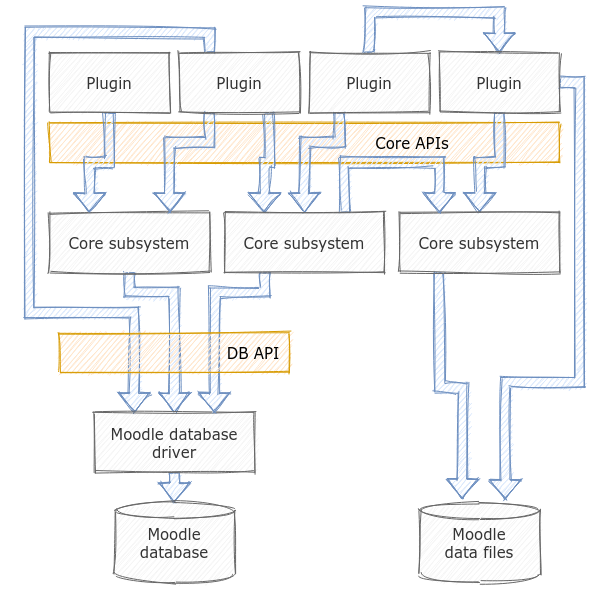
\includegraphics[scale=0.7]{Fejezetek/Images/moodleBuild.png}
\end{center}

\subsection{A pluginek fajtái}

Jelenleg a Moodle-ben 58 fajta plugin létezik, mind teljesen különböző funkcionalitással és szerkezettel. Ezeket a mapparendszerben lévő elhelyezkedésükkel különböztetjük meg egymástól. A plugineken belül lehetnek további típusú pluginek, amelynek a közös tulajdonsága, hogy az alapplugint használja, ezeket a mappán belüli másik mappa fogja meghatározni. Például, ha szeretnénk egy olyan plugint készíteni, amely minden alkalommal a felhasználó kezdőfelületére kiírja egy dobozba, hogy "Hello User", akkor az egy block típusú plugin lesz, és a mapparendszerben a blocks/hellouser mappába kell létrehozni. Néhány plugin köztük fontosabb, többször használtabb, vannak viszont olyanok, amelyek speciálisabbak. Például az Activity modules az egyik legfontosabb, ez maga az oktatási felületet biztosító plugin, így ennek több alpluginja lehet, mint például a Calendar type pluginnak. Néhány fontosabb plugin: 
\begin{itemize}
    \item Activity Module (oktatás, osztályzás), 
    \item Blocks(Alap felület variálása, új állandó tartalom megjelenítése), 
    \item Themes( oktatási felület kinézete, nem csak CSS segítségével), 
    \item Authentication (Regisztráció, bejelentkezés), 
    \item Enrolement (Rangok kiosztása, kurzusok személyeinek beállítása), 
    \item Course (kurzus létrehozása, tananyag feltöltése, tesztek létrehozása), 
    \item Admin (Pluginek kezelése, menedzselése, testreszabása, telepítése és törlése), 
    \item Local (Saját személyes pluginek kezelése, létrehozása) 
\end{itemize}

Természetesen minden plugin, amit a \href{https://moodle.org/plugins/}{Moodle Plugin website}-ról töltünk le, az a Local mappában kerül telepítésre, így a szakdolgozat mappaszerkezete is a local/szakdolgozat formát követi.

\section{Moodle plugin}

\subsection{Közös elemek}

Minden Moodle plugin tartalmaz 3 elemet:
\begin{itemize}
    \item version.php
    \item lang/en/plugintípus\_pluginnév.php
    \item db/install.xml
\end{itemize}

Ezek nélkül a Moodle fel sem telepíti a pluginünket. A version.php felel a pluginek tulajdonságainak meghatározásában, amelyek segítségével ismeri fel a Moodle a különböző modulokat. Két adatot kötelező megadni ebben: a \$plugin->component tartalmazza a plugin azonosítóját, amely mindig a plugintípus\_pluginnév formátum, a másik a \$plugin->version, amely a plugin verziószámát tartalmazza az alábbi formában: YYYYMMDDXX, ahol a YYYY az aktuális évet, az MM az aktuális hónapot, a DD pedig a napot tartalmazza, az XX pedig a jelenleg futó verziószámot, amely mindig 01-gyel kezdődnie. A verziókról később írok részletesen. Egyéb tulajdonságok, amelyeket a version.php-ben határozunk meg:
\begin{itemize}
    \item \$plugin->requires: minimum Moodle verziószám
    \item \$plugin->supported: ajánlott Moodle verziószám
    \item \$plugin->release: mely Moodle verzióra érkezett a plugin
    \item stb.
\end{itemize}

A lang/en/plugintípus\_pluginnév.php tartalmazza azokat a szövegeket, amelyek felhasználunk a plugin elkészítésében. Ezek segítségével nem kell a kódba beleégetni a különböző kiírásokat és feliratokat, hanem ebből a fájl-ból kiolvasva történik meg a behelyettesítés. Ennek a lehetőségnek hála tudunk akár többnyelvű modult létrehozni. Az alapja egy tömb, melyben kulcsként a kulcsszót adjuk meg, értékként megint a megjeleníteni kívánt szöveget. Az index.php-ben pedig a get\_string() metódus segítségével tudjuk kiolvasni. Alapból a Moodle csak az angol nyelvet telepíti fel, így ha szeretnénk magyar nyelvet belerakni, akkor a Site Administration/Administration/Language/Language packs belül kell telepíteni, illetve a lang mappában kell létrehozni egy /hu/plugintípus\_pluginnév.php fájlt és megcserélni az en-ben lévő \$string[] értékeit magyarra. \par

Az utolsó fájl pedig a db/install.xml. Ez a fájl kakukktojás a másik kettőhöz képest, mert ennek a megléte nem szükséges a plugin létrehozásához. Célja, hogy a pluginhez tudjunk táblázatot készíteni, annak pedig az oszlopait és annak értékeit meghatározza. Ezenkívül a fájl tartalmazza még a plugin útvonalát. Amikor telepítjük a plugint, akkor a Moodle adatbázisához hozzáteszi ezt az adatbázist mdl\_plugintípus\_pluginnév néven. Viszont ügyelni kell a plugin törlése esetén az adatbázisban lévő adatok is törlődnek, így biztonsági mentést érdemes végezni, mielőtt eltávolítanánk a saját modulunk.\par

Ezek a legfontosabb közös elemei egy pluginnek, ezenkívül még létezik néhány:
\begin{itemize}
    \item classes/ mappa, amely a pluginben felhasználni kívánt egyedi osztályokat tartalmazza
    \item styles.css, amely az index.php-hoz tartozó css
    \item readme fájl
    \item lib.php, amely az index.php-ban felhasznált függvények tárolására szolgás
    \item stb.
\end{itemize}

\subsection{Dinamikus plugin készítése és főbb elemei}

A Moodle korábban létrejött, mint azok a modern PHP keretrendszerek, amelyek tartalmazzák a a HTTP kérések kezelését és irányítását és létrehozzák a válaszokat is a kérésekkel. Emiatt a Moodle a Page Controller minta segítségével valósítja meg ezt a folyamatot. Ennek működése, hogy minden request egy request handler-en keresztül történik feldolgozásra és innen irányítja tovább a megfelelő könyvtárakba, ahol a feldolgozás és megvalósítás történik, majd a response-t is a request handleren keresztül válaszol a felhasználó számára. A requestek a címsorban történnek tárolásra és ezen keresztül történnek a könyvtárakban az értékadások. Az alábbi illusztráció jól bemutatja a folyamatot:
\begin{center}
    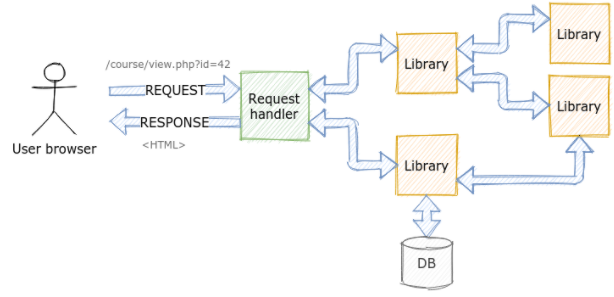
\includegraphics[scale=0.8]{Fejezetek/Images/requestHandler.png}
\end{center}

Ezen keresztül lehet látni, hogy az $id$ adattag megkapja a $42$ értéket, a könyvtárak ezen keresztül lefuttatják a megfelelő függvényeket és a választ a request handleren keresztül közlik a felhasználóval. Hogy el tudjuk érni a request handler-t szükséges elsőnek betölteni a főmappában lévő config.php fájl-t, amely az alábbi parancs segítségével történik: \par
\hfill \break
require(\_\_DIR\_\_. '/../../config.php');
\hfill \break

Ez a fájl tartalmazza az adatbázis, session-ök, jelenlegi kurzusok, témák és nyelvek inicializálását és ezekhez kapcsolódó adattagokat, funkciókat. Pontosítva, a config.php-n keresztül történik a többi főbb php file meghívásra, melyeken keresztül tudjuk a Moodle főbb részeit elérni. \par

Ezenkívül biztonsági okokból a fejlesztő nem tudja elérni a \$\_GET,  \$\_POST és  \$\_REQUEST paramétereit, helyette a Moodle biztosít egy require\_param() és optional\_param() függvényeket. Ezek meghívásával tudjuk a megfelelő adattagnak a címsorban lévő értéket felvetetni. A függvényeknek meg kell adni a címsorban szereplő kulcsszót, amely alapján veszik fel az értéket (A példánkban ez az $id$ volt), egy kezdőértéket, ha nem találna ilyet és egy típust, hogy milyen értéket vegyen fel. Ezekből rengeteg típus van, a leggyakoribbak:

\begin{itemize}
    \item PARAM\_INT: Integert váró paraméter
    \item PARAM\_ALPHA: ASCII kódolású, csak betűkből álló rövid stringet vár bemenetnek
    \item PARAM\_ALPHANUM: ASCII kódolású, betűkből és számokból álló rövid stringet vár bemenetnek
    \item PARAM\_BOOL: Egy 0-át vagy 1-et visszaadó érték, mely ha 'off'-t, 'no'-t vagy 'false'-t kap, akkor ad vissza 0-t, ha 'on'-t, 'yes'-t vagy 'true'-t kap, akkor pedig 1-et.
    \item PARAM\_TEXT: UTF-8at támogató nyelv, minden taget lecsupaszítva
    \item PARAM\_PATH: egy úgyvonalat ad vissza.
\end{itemize}

Az összes ilyen típust a lib/moodlelib.php-ben lehet megtalálni és ott vannak a megfelelő tisztító és vezérlőkódok is leprogramozva.

A másik fontos része a pluginünknek, hogy azt a böngésző címsorából közvetlenül ne tudjuk elérni vagy módosítani, hanem csak a könyvtárakon keresztül tudjuk betölteni, ehhez az alábbi sornak kell a kódban lennie: \par
\hfill \break
defined('MOODLE\_INTERNAL') || die();
\hfill \break

Ennek segítségével tudjuk megcsinálni, hogy vagy csak a Moodle könyvtár segítségével történjen a betöltés, ha pedig nem sikerült úgy, abban az esetben egy fehér képernyő látszódjon és a console-ból se lehessen kiolvasni semmilyen forráskódot. \par
Minden egyéb betöltést pedig a /classes mappából történik. 

\subsection{Plugin megjelenítése}

Minden Plugin kezdőfelülete az index.php. Ebben hozzuk létre a változóinkat, adunk nekik értéket, jelenítjük meg a plugin tartalmát, és itt állítunk be témát. Minden pluginhez tartozik egy \$PAGE globális változó, amelyen keresztül készítjük el és szabjuk testre a plugint. Egy \$PAGE esetén sok tulajdonságot lehet beállítani, viszont első körben nézzük meg a legfontosabbakat. \par
Elsőnek állítsuk be a \$PAGE URL címét: 
\hfill \break
\$PAGE->set\_url(new moodle\_url('/plugintípus/pluginnév/index.php));
\hfill \break

Ezzel a függvényhívással már tudunk hivatkozni a jelenlegi címre, illetve a plugin indításakor a Moodle tudni fogja, hogy melyik címet kell megnyitnia. Később is hasznos lehet nekünk ez, mivel például ha szeretnénk egy form-ot létrehozni, akkor a fejléc lehet az alábbi:
\hfill \break
echo '<form method="get" action="'.\$PAGE->url.'">';
\hfill \break

A másik nagyon fontos, hogy megadjuk, hogy a \$PAGE mihez tartozik, a Moodle mely részével van összekötve, összekapcsolva. Itt értem ez alatt, hogy plugin egy modulhoz, egy kurzushoz vagy magához a rendszerhez van készítve, azon részeivel van kapcsolatban. Ezt a következő módon tudjuk megvalósítani:

\hfill \break
\$PAGE->set\_context(context\_system::instance());
\hfill \break

Ebben az esetben egy rendszerszintű plugint fogunk érteni. Ha kurzushoz akarjuk, akkor paraméternek a contect\_course::instance(\$kurzusid)-t, ha pedig egy modulhoz, akkor a contect\_module::instance(\$moduleid)-t kell megadni. \par

Ezeket kötelező beállítani minden \$PAGE esetén, de vannak még olyan tulajdonságok, amelyek fontosak. A
\hfill \break
\$PAGE->set\_title(get\_string('pluginname', 'plugintípus\_pluginnév'));
\hfill \break
segítségével a böngésző tetején a füleknek a nevét lehet beállítani, itt is a lang/en/plugintípus\_pluginnév-ből veszi ki a pluginname kulcsú értéket és azt állítja be, a 
\hfill \break
\$PAGE->set\_heading(get\_string('heading', 'plugintípus\_pluginnév'));
\hfill \break
segítségével tudunk címet adni a pluginnak, ez is ugyannazzal a módszerrel történik, mint a title esetén, végül pedig a
\hfill \break
\$PAGE->set\_pagelayout('standard');
\hfill \break
függvényhívás segítségével tudjuk kiválasztani, hogy mely beépített alapkinézetet szeretnénk választani. Nagy többségében a 'standard' kinézetet választják, de ebből is többféle létezik: 'base','course','admin','login',stb. \par

Ha pedig mindent sikerült beállítani, akkor ezeket már csak ki kell írni a képernyőre. Ebben segít a \$OUTPUT változó, amely a renderelésért felel, ezen változó függvényeinek meghívásával történnek meg a kiíratások, megjelenítések. Például eddig bemutatott \$PAGE adattagok értékeit beállítottuk, ennek megjelenítésére a 
\hfill \break
echo \$OUTPUT->header();
\hfill \break
meghívásával tudjuk megjeleníteni. A lábléc-et az
\hfill \break
echo \$OUTPUT->footer();
\hfill \break
parancs szükséges, viszont a index.php "törzséhez" nem kell külön az \$OUTPUT változó egy függvényét meghívni, elég ha megfelelő echo és html tagek közt megadjuk. Viszont célszerű speciális esetekben a Moodle által létrehozott kiírató függvényeket használni. Ezeket az eseteket a következő ábra bemutatja:

\begin{center}
    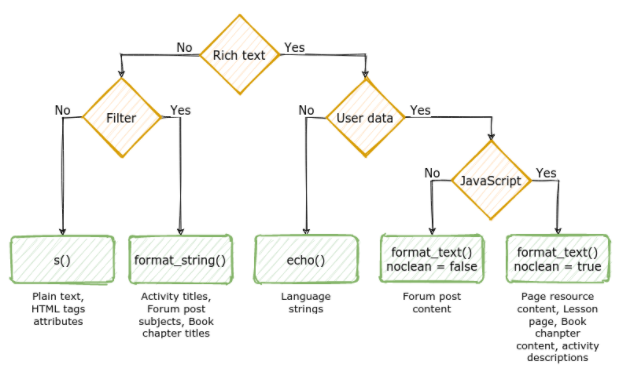
\includegraphics[scale=0.9]{Fejezetek/Images/print.png}
\end{center}

Ezenkívül lehetőségünk van különböző HTML megjelenítést és logikai elkülönítést segítő függvényeket is meghívni, ezt a html\_writer osztály-ban lévő függvények segítségével tudjuk megtenni. Például
\hfill \break
echo html\_writer::tag('input','nev',[ 'type' => 'text', 'name' => 'username']); 
\hfill \break
kiíratás segítségével egy új input taget tudubk létrehozni, amely szöveget vár, username néven tárolja el és a kezdőértéke a nev szöveg. Ilyen függvényekből is több fajta létezik: link(), img(), table(), stb.

\subsection{Egyéb beállítások}

A Moodle-ben van lehetőségünk még rengeteg dologra egy plugin készítésével kapcsolatban. Lehet
\begin{itemize}
    \item Fő menüsorra elhelyezni, vagy almenüsorra beszúrni,
    \item Admin felhasználói beállításokat lehet adni, amelyek segítségével irányítható a plugin,
    \item Verziókövetés, 
    \item Adatbázist lehet hozzákapcsolni és abból SQL lekérdezések segítségével lehet az adatokat kinyerni,
    \item stb.
\end{itemize}

Ezekkel azért nem foglalkozunk komolyabban, mivel a szakdolgozat nem dolgozza fel, így csak említés és rövid áttekintésként vesszük végig. \par

A menübár egy fa struktúrával felépített UI amelynek 3 részét különböztetjük meg:
\begin{itemize}
    \item Navigálásért szolgáló bár, amely a kurzusok, órák és ahhoz tartozó oldalak között lehet lépegetni.
    \item Jelenlegi bár, amely az aktuális bárt jeleníti és tárolja
    \item Beállítás bár, amely egy kurzushoz, órához, stb.-hez tartozó beállítások és funkciók megjelenítésével foglalkoznak.
\end{itemize}

Ha szeretnénk az oldalhoz menüsort beállítani, azt a \$PAGE->navigation->add() függvény meghívásával tudjuk megtenni, amelybe egy linket kell belemásolni, illetve ha szeretnénk saját menübárt, akkor azt a lib.php fájlban kell függvények formájában implementálni. Ha pedig szeretnénk a főoldalon található navigation bar-ba elhelyezni, akkor az alábbi kódot kell a lib.php-ban elhelyezni: 

\begin{lstlisting}
/**
 * Add link to index.php into navigation drawer.
 *      
 * @param global_navigation $root Node representing the global navigation tree.
 */
function /plugintipus_pluginnev_extend_navigation(global_navigation $root) {

    $node = navigation_node::create(
        get_string('sayhello', 'plugintipus_pluginnev'), 
        new moodle_url('/plugintipus/pluginnev/index.php'),
        navigation_node::TYPE_CUSTOM,
        null,
        null,
        new pix_icon('t/message', '')
    );
    $node->showinflatnavigation = true;

    $root->add_node($node);
}
\end{lstlisting}

Az adminisztrátori beállításokat a settings.php-ban kell létrehozni, a fejlesztői beállításokat a config.php-ban. Ezek alapján könnyebben szét lehet szedni, hogy melyek a plugin tényleges működése és melyek annak tesztelésére szolgálnak. A configban történt módosításokat és adattagok értékeinek tárolására a config tábla van fenttartva és a \$CFG adattagban történik a meghívása. Ebben tudjuk a get\_config() és set\_config() segítségével lekérni és módosítani. Az adminisztrációs beállítások az admin\_category fa struktúrájú objektumban tárolódnak, melynek a gyökéreleme az \$ADMIN objektum és ezen keresztül tudjuk lekérni változókat. \par

A verziókövetés a version.php file-ban történik. Miven verziószám az alábbi alakban nézz ki YYYYMMDDXX. Ha történik valamilyen szignifikáns változtatás, például adatbázisséma változás, egy új adatbázis létrehozása vagy új elem hozzáadása, akkor léptetni kell a verziószámot egyaránt. A Moodle-ben nincs arra lehetőség, hogy a verziószámot csökkentsük, mindig a következő verziónak "nagyobbnak" kell lennie, mint az aktuális. A nagyobb alatt azt értjük, hogy vagy a dátumnak kell frissebbnek lennie, mint az előző verziószámban lévő, vagy ha a dátum megegyezik, akkor az XX helyén lévő számnak kell nagyobbnak lennie az előzőnél. Ezenkívül az XX helyén lévő számok segítségével tudunk új irányutakat létrehozni a plugin fejlesztésében. \par

Végezetül pedig adatbázisokat lehet egy pluginhez hozzákapcsolni, azon keresztül szerkeszteni és lekérdezéseket indítani. A Moodle-ben egy adatbázis létrehozásához és módosításához létrehozott egy XMLDB editort, hogy azon keresztül generáljon XML fájlokat és azok megfeleljenek a Moodle-ben használt szabályoknak. Ezt a Portálkezelés -> Fejlesztés -> XMLDB-szerkesztő-n keresztül tudjuk elérni. Ezekhez tartozó szabályokból sok van, néhány közülük:

\begin{itemize}
    \item Minden táblának a neve az alábbi módon kell kinéznie: plugintípus\_pluginnév\_tárolniKívántAdat.
    \item Minden táblának kell lennie egy automatikusan léptetett számlálóval.
    \item Minden tábla nevének hossza maximum 28 karakter.
    \item Minden oszlop nevének hossza maximum 30 karakter.
    \item Minden tábla- és oszlopnévnek kerülnie kell a Moodle-ben létrehozott kulcsszavakat.
    \item stb.
\end{itemize}

Minden adatbázis a \$DB változóban. Ehhez include-olni kell a gyökérkönyvtárban található config.php file-t. Ezen a változón keresztül lehet indítani táblázatmódosításokat és lekéréseket. Rengeteg előre gyártott függvénnyel rendelkezik, mint például a get\_records\_sql(), count\_records(), record\_exists és így tovább. 
\chapter{Moodle plug-in készítés folyamata}

\section{Előzetes ötletek, első lépések}

Első körben érdemes definiálni, hogy mit kell tudnia a pluginnek és így milyen fajta pluginre lesz szükség. Tudjon
\begin{itemize}
    \item Feladat nehézségeket kiválasztani,
    \item Feladat nehézség szerint tudjon feladatot generálni,
    \item A felhasználótól tudjon lekérni megoldást,
    \item A feladat megoldását összevetve a felhasználó megoldásával tudja megjeleníteni.
\end{itemize}

Ehhez nem szükséges speciálisabb plugint kiválasztani, elég, ha local. Ezután alkossuk meg a kötelező fájlokat. A lang\_en\_local\_szakdolgozat első sorába írjuk be az alábbi sort:

\begin{lstlisting}[language=php]
$string['pluginname'] = 'Normalization';
\end{lstlisting}

Ezzel kész is fejléc címe. Ezután hozzuk létre a version.php-t, amelybe az alábbi sorokat tegyük:

\begin{lstlisting}[language=php]
$plugin->component = 'local_szakdolgozat';
$plugin->version = 2021013000;
\end{lstlisting}

És már csak indítsuk újra a Moodle-t, ekkor felismeri a plugint és feltelepíti. Ezután pedig készítsük el az index.php-t, a classes mappát és a mappába másoljuk be a Relációsémákat generáló és megoldó osztályokat.

\section{A plugin felépítése}

A pluginnak 4 része lesz:
\begin{enumerate}\setcounter{enumi}{-1}
    \item Fejléc megalkotása
    \item Nehézség kiválasztása
    \item Feladat generálása
    \item Megoldás megjelenítése
\end{enumerate}

Elsőnek beállítjuk az url-t, a címet,a kapcsolódását a moodle-hez, a fejléc szövegét, és milyen kialakítású legyen.
Ezenkívül meghívjuk a saját osztályainkat, illetve a gyökérkönyvtárban lévő config.php-t, mivel szükségünk lesz a \$PAGE, illetve a \$OUTPUT változókra. 
\begin{lstlisting}
<?php

require(__DIR__. '/../../config.php');
require_once('classes/Relaciosema.php');

$PAGE->set_url(new moodle_url('/local/szakdolgozat/index.php'));
$PAGE->set_context(context_system::instance());
$PAGE->set_title(get_string('pluginname', 'local_szakdolgozat'));
$PAGE->set_heading(get_string('heading', 'local_szakdolgozat'));
$PAGE->set_pagelayout('standard');

echo $OUTPUT->header();
\end{lstlisting}

A nehézség kiválasztása egy egyszerű nyomógombos megoldás, kezdeti értéknek az egyszerű megadva. Amelyiket kiválasztja a felhasználó, arról fog kapni egy feladatot. A nehézség mentése az urlben történik és egy \$difficulty változóval történik a kiolvasása. \par

A Feladat generálása előtt egy felirat található, ahol egy leírás található, hogy milyen formában kell beküldeni a megoldást. Ez azért fontos, hogyha egy megoldást és egy felhasználói választ akarunk összeegyeztetni, akkor elsőnek érdemes átalakítani egy felhasználói választ egy Relációséma példánnyá, így könnyebben tudjuk kezelni. A feladat generálás után pedig 
\chapter{Függelék}

\section{A program forráskódja}
A függelékbe kerülhetnek a hosszú táblázatok, vagy mondjuk egy programlista:
% A verbatim kornyezet hasznalatanal ügyeljünk rá, hogy az editor a szóközöjket át ne írja tab karakterekre!
\begin{verbatim}
   while (ujkmodosito[i]<0)
   {
      if (ujkmodosito[i]+kegyenletes[i]<0)
      {
         j=i+1;
         while (j<14)
         if (kegyenletes[i]+ujkmodosito[j]>-1) break;
         else j++;
         temp=ujkmodosito[j];
         for (l=i;l<j;l++) ujkmodosito[l+1]=ujkmodosito[l];
         ujkmodosito[i]=temp;
      }
      i++;
   }
\end{verbatim}
\chapter*{Nyilatkozat}
%Egy üres sort adunk a tartalomjegyzékhez:
\addtocontents{toc}{\ }
\addcontentsline{toc}{section}{Nyilatkozat}
%\hspace{\parindent}

% A nyilatkozat szövege más titkos és nem titkos dolgozatok esetében.
% Csak az egyik tipusú myilatokzatnak kell a dolgozatban szerepelni
% A ponok helyére az adatok értelemszerûen behelyettesídendõk es
% a szakdolgozat /diplomamunka szo megfeleloen kivalasztando.


%A nyilatkozat szövege TITKOSNAK NEM MINÕSÍTETT dolgozatban a következõ:
%A pontokkal jelölt szövegrészek értelemszerûen a szövegszerkesztõben és
%nem kézzel helyettesítendõk:

\noindent
Alulírott \makebox[4cm]{\dotfill} szakos hallgató, kijelentem, hogy a dolgozatomat a Szegedi Tudományegyetem, Informatikai Intézet \makebox[4cm]{\dotfill} Tanszékén készítettem, \makebox[4cm]{\dotfill} diploma megszerzése érdekében.

Kijelentem, hogy a dolgozatot más szakon korábban nem védtem meg, saját munkám eredménye, és csak a hivatkozott forrásokat (szakirodalom, eszközök, stb.) használtam fel.

Tudomásul veszem, hogy szakdolgozatomat a Szegedi Tudományegyetem Informatikai Intézet könyvtárában, a helyben olvasható könyvek között helyezik el.

\vspace*{2cm}

\begin{tabular}{lc}
Szeged, \today\
\hspace{2cm} & \makebox[6cm]{\dotfill} \\
& aláírás \\
\end{tabular}

\vspace*{4cm}


\chapter*{Köszönetnyilvánítás}
\addcontentsline{toc}{section}{Köszönetnyilvánítás}
Első körben szeretném megköszönni családomnak, hogy támogattak egész tanulmányaim alatt, illetve motiváltak a nehezebb napokon. Szeretném megköszönni a barátaimnak, akik a monoton munkából kizökkentettek és így tették könnyebbé mindennapjaim. Szeretném megköszönni a tanáraimnak, illetve csoporttársaimnak, hogy segítséget nyújtottak az egyetemi tanulmányaim alatt.
Ezenkívül külön szeretném megköszönni Dr. Németh Gábornak, hogy vállalt és segített engem.

\newpage
%% Az itrodalomjegyzek keszitheto a BibTeX segedprogrammal:
%\bibliography{diploma}
%\bibliographystyle{plain}

%VAGY "kézzel" a következõ módon:

\begin{thebibliography}{9}
%10-nél kevesebb hivatkozás esetén

%\begin{thebibliography}{99}
% 10-nél több hivatkozás esetén

\addcontentsline{toc}{section}{Irodalomjegyzék}

%Elso szerzok vezetekneve alapjan ábécérendben rendezve.


%folyóirat cikk: szerzok(k), a folyóirat neve kiemelve,
%az evfolyam felkoveren, zarojelben az evszam, vegul az oldalszamok es pont.
\bibitem{normalcikk}
Moussa Demba,
Algorithm for relational database normalization up to 3NF
\emph{International Journal of Database Management Systems}, \textbf{5}(2013), 39--51.
\href{http://airccse.org/journal/ijdms/papers/5313ijdms03.pdf}{http://airccse.org/journal/ijdms/papers/5313ijdms03.pdf}

%könyv (szerzo(k), a könyv neve kiemelve, utana a kiado, a kiado szekhelye, az evszam es pont.)
\bibitem{adatb}
Dr. Balázs Péter, Dr. Németh Gábor
\emph{Adatbázisok a tervezéstől az alkalmazásfejlesztésig},
Szegedi Tudományegyetem, Szeged, 2019.
\href{http://eta.bibl.u-szeged.hu/3387/1/BalazsNemeth_Adatbazisok_jegyzet_2019.pdf}{http://eta.bibl.u-szeged.hu/3387/1/BalazsNemeth\_Adatbazisok\_jegyzet\_2019.pdf}

\bibitem{MoodleDev}
The Moodle Development Team.
\emph{Moodle Developer Documentation (Version 3.10)} 2021. \href{https://docs.moodle.org/dev/Tutorial}{https://docs.moodle.org/dev/Tutorial}

\bibitem{MoodleTutorial}
Learnmoodle
\emph{Massive Open Online Courses.} 
\href{https://learn.moodle.org/}{https://learn.moodle.org/}

\bibitem{ricsidoga1}
Korom Richárd, Dr. Németh Gábor
\emph{Adatbázis modellezés és SQL feladatok automatikus kiértékelése gráfelméleti alapokon},
Szegedi Tudományegyetem, Szeged, 2019.
\href{https://www.inf.u-szeged.hu/sites/default/files/koromrichard_tdka2020o.pdf}{https://www.inf.u-szeged.hu/sites/default/files/koromrichard\_tdka2020o.pdf}

\bibitem{ricsidoga2}
Korom Richárd, Dr. Németh Gábor
Adatbázis modellek automatikus kiértékelése – az első verzió\hfill \break
\emph{$26^{th}$ Multimedia in Education Online Conference}, \textbf{5}(2020), 90--92.
Szegedi Tudományegyetem, Szeged, 
\href{https://www.mmo.njszt.hu/Kiadvanyok/2020/MMO2020_Proceedings.pdf}{https://www.mmo.njszt.hu/Kiadvanyok/2020/MMO2020\_Proceedings.pdf}

\end{thebibliography}


\end{document}
